% %%
\documentclass[lettersize,journal]{IEEEtran}
%\documentclass[lettersize,journal,draft]{IEEEtran}

\usepackage{amsmath,amsfonts,amssymb}
\usepackage{algorithmic}
\usepackage{array}
\usepackage{textcomp}
\usepackage{stfloats}
\usepackage{url}
\usepackage{verbatim}
\usepackage{graphicx}
\usepackage{balance}
\newtheorem{theorem}{Theorem}
\newtheorem{proposition}{Proposition}
\newtheorem{lemma}{Lemma}
\newtheorem{corollary}{Corollary}
\newtheorem{remark}{Remark}
\newtheorem{assumption}{Assumption}
\hyphenation{op-tical net-works semi-conduc-tor IEEE-Xplore}
\def\BibTeX{{\rm B\kern-.05em{\sc i\kern-.025em b}\kern-.08em
    T\kern-.1667em\lower.7ex\hbox{E}\kern-.125emX}}

\urlstyle{same}
\begin{document}

\title{Adaptive Navigation along the Separatrix and Okubo-Weiss Boundary of the Double Gyre}

\author{Christopher Waight, Christopher A. Kitts \IEEEmembership{Senior Member, IEEE}
\thanks{Manuscript received Month Day, Year; revised Month Day, Year.}
\thanks{C. Waight is a PhD Candidate in the Robotic Systems Laboratory, Department of Mechanical
Engineering, Santa Clara University, Santa Clara, CA 95053 USA (e-mail: cwaight@scu.edu)}
\thanks{C. A. Kitts is Professor and Director of the Robotic Systems Laboratory, Department of
Mechanical Engineering, Santa Clara University, Santa Clara, CA 95053 USA (e-mail: ckitts@scu.edu)}
}
\markboth{Journal of \LaTeX\ Class Files,~Vol.~XX, No.~X, Month~Year}%
{Waight, Kitts \MakeLowercase{\textit{et al.}: Adaptive Navigation along the Separatrix and Okubo-Weiss Boundary of the Double Gyre}}

\maketitle

% ---------------------------------------------------------------------------
\begin{abstract}
Objective Eulerian coherent structures (OECSs) are short-term,
frame-invariant transport barriers that organize instantaneous material
transport in general dynamical systems. They can be viewed as the
instantaneous counterparts of stable and unstable manifolds, extracted
from the rate-of-strain field at a single instant rather than from
trajectories integrated over a finite horizon. Identifying OECSs is
useful for applications that demand short-term or real-time forecasting,
including oceanography and weather prediction. In this paper, we present
a collaborative robotic control strategy that tracks the short-term
attracting and repelling structures of a flow, including ocean flows,
without prepositioning the robots and without requiring global
information about the dynamics; it relies instead on local sensing,
prediction, and correction. For the two-dimensional incompressible flows
we consider, the sign of the determinant of the flow Jacobian,
equivalently the Okubo-Weiss field, partitions the flow into
vorticity-dominated and strain-dominated regions: its zero level set
forms the boundary between them, and its trench marks the strongest
hyperbolicity, where the hyperbolic OECS resides. We develop two
complementary tracking modes. In the first, the team follows the
Okubo-Weiss boundary, the zero level set that divides the two regimes.
In the second, the team navigates the Jacobian-determinant field itself.
Rather than steepest descent or ascent, a modified Newton step, which
reweights the search directions so the team snaps onto the trench more
rapidly, drives the team along the structure, through a saddle point of
this scalar field, and down the opposing branch. The strategy is
implemented with a team of six robots and validated on a time-dependent
model of a wind-driven double-gyre flow and on actual ocean-flow data.
We present simulation results and discuss theoretical guarantees of the
collaborative tracking strategy.
\end{abstract}

\begin{IEEEkeywords}
Multirobot Systems, Adaptive Navigation, Vector Fields, Okubo-Weiss, Separatrix,
Double Gyre, Critical Points, Cooperative Estimation, Cluster Control
\end{IEEEkeywords}


% ---------------------------------------------------------------------------
\section{Introduction}
\label{sec:intro}

\IEEEPARstart{M}{ultirobot} systems operating in geophysical flows such as ocean currents and
atmospheric jets often need to locate and track dynamically meaningful boundaries
rather than isolated critical points. Two such boundaries appear prominently in
steady two-dimensional flows: the separatrix, which contains both the stable and unstable manifold connecting to saddle points, which partitions the domain into two distinct basins; and the
Okubo-Weiss boundary, the locus of points where the local flow transitions from
rotation-dominated to strain-dominated behavior. Both structures are relevant to
dispersion modeling, pollutant containment, and the deployment of sensor networks
in coastal and atmospheric environments [1, 2, 3].

Prior work on multirobot navigation in physical vector fields has addressed
gradient-following in scalar fields [4, 5] and critical point estimation in
vector fields using three-robot formations [6]. These methods provide convergence
to isolated features such as sinks, vortices, and saddle points, but do not
address navigation along one-dimensional manifolds or closed-curve boundaries
within the field. Tracking such structures requires estimating not only the
Jacobian at the cluster centroid but also its spatial derivatives.



This paper presents the following contributions:
\begin{enumerate}
    \item A distributed quadratic estimator that uses simultaneous measurements
          from six omnidirectional robots to recover the Jacobian $\mathbf{J}$,
          the determinant $\det(\mathbf{J})$, its gradient
          $\nabla\det(\mathbf{J})$, and its Hessian $\mathbf{H}_D$ at the cluster
          centroid, with no prior knowledge of the field.
    \item Two adaptive controllers presented in parallel: (a) a hybrid three-mode
          separatrix tracker (Logic C) that uses the eigenbasis of
          $\mathbf{H}_D$ to slide along the stable manifold of the double-gyre
          saddle; (b) an Okubo-Weiss boundary tracker that applies a Newton-step
          contour-following law to drive $\det(\mathbf{J}) \to 0$ while drifting
          tangentially along the boundary.

    \item Monte Carlo simulation validation of both controllers under a fully
          specified noise model, with success-rate maps over a two-dimensional
          sweep of measurement and position noise standard deviations.

    \item Demonstration of effectiveness on real world oceanic data.
\end{enumerate}

The remainder of the paper is organized as follows. The rest of this
section reviews related work. Section~\ref{sec:detj_field} formulates the
problem, describing the double-gyre model, the $\det(\mathbf{J})$ field, and
the separatrix as an Eulerian trench.
Section~\ref{sec:estimation} develops the six-robot quadratic estimator
and its sensitivity. Section~\ref{sec:controllers} presents both adaptive
controllers.
Section~\ref{sec:stability} provides stability proofs.
Section~\ref{sec:methods} describes the simulation program, noise model, and
testing plan. Section~\ref{sec:results} presents results.
Section~\ref{sec:discussion} discusses implications and failure modes.
Sections~\ref{sec:limitations} and \ref{sec:future} cover limitations and
future work. Section~\ref{sec:conclusion} concludes.


% ---------------------------------------------------------------------------

\subsection{Lagrangian Coherent Structures and FTLE}

% TODO: 4-6 sentences. Cover: Haller's LCS framework, finite-time Lyapunov
% exponents (FTLE) as a Lagrangian tool for identifying ridges of maximal
% stretching that approximate stable and unstable manifolds. Note that FTLE
% computation requires integrating particle trajectories, making it unsuitable
% for real-time onboard estimation. Contrast with the Eulerian approach used
% in this paper.
% Key references: Haller [1], Peacock and Haller [2], Shadden double gyre [3].

\subsection{Eulerian Indicators: Okubo-Weiss, Q-Criterion, Hua-Klein}

% TODO: 4-6 sentences. Cover: Okubo (1970) and Weiss (1991) independently
% proposed $Q = (s_n^2 + s_s^2 - \omega^2)/4$ as a pointwise indicator;
% $Q < 0$ (or equivalently $\det(\mathbf{J}) > 0$) characterizes
% rotation-dominated regions. The Q-criterion of Hunt (1988) generalizes to
% 3D. Hua and Klein (1998) refined the Okubo-Weiss criterion for oceanographic
% use. Cite all four; explain the sign convention used in this paper
% ($\det(\mathbf{J}) > 0 \Leftrightarrow$ rotation-dominated).
% Note that all Eulerian indicators require only instantaneous field measurements,
% unlike FTLE. Cite Okubo [7], Weiss [8], Hua and Klein [9].

\subsection{Distributed Sampling and Hessian Estimation}

% TODO: 4-6 sentences. Cover: Ögren, Fiorelli, Leonard on cooperative gradient
% climbing [10]; Briñón-Arranz, Renzaglia, Schenato on symmetric formations for
% gradient and Hessian estimation [11]; Kitts and Mas cluster space control [12];
% McDonald, Kitts, Neumann on scalar field navigation primitives [4].
% Note that Hessian estimation in scalar fields (4 or more robots) is well studied,
% but quadratic estimation in vector fields (requiring 6 robots for exact
% determination of both u and v) has not previously been reported.

\subsection{Cluster Space Control and SAS Formations}

% TODO: 3-4 sentences. Cover: Kitts and Mas (2009) cluster space specification
% and control [12]; Adamek, Kitts, Mas (2014) gradient-based navigation for
% surface vessels [13]; prior work on three-robot and four-robot SAS formations
% for vector field navigation [6]. Connect the six-robot pentagon-of-pairs
% formation used here to the lineage of SAS cluster designs.


% ---------------------------------------------------------------------------
\section{Problem Formulation}
\label{sec:detj_field}

\subsection{Flow Fields and Local Polynomial Models}

A planar flow assigns a velocity vector $\mathbf{v}(\mathbf{p}) =
(u(\mathbf{p}), v(\mathbf{p}))$ to each position $\mathbf{p} = (x, y)$ in its
domain. Its Jacobian at $\mathbf{p}$ is
\begin{equation}
    \mathbf{J}(\mathbf{p}) =
    \begin{bmatrix}
        \partial u / \partial x & \partial u / \partial y \\
        \partial v / \partial x & \partial v / \partial y
    \end{bmatrix},
    \label{eq:jacobian}
\end{equation}
and we write $D(\mathbf{p}) = \det(\mathbf{J}(\mathbf{p}))$ throughout.

In prior work [6], a three-robot cluster fit a linear model to each
component of $\mathbf{v}$, assembled the estimated Jacobian
$\mathbf{J}$ and offset $\mathbf{h}$, and recovered the critical point
$\mathbf{p}^* = -\mathbf{J}^{-1}\mathbf{h}$ where $\mathbf{v}(\mathbf{p}^*) =
\mathbf{0}$, together with its type from the eigenvalues of $\mathbf{J}$.
A linear model, however, carries no information about how $\mathbf{J}$
itself varies in space. The structures addressed in this paper, boundaries
between rotation-dominated and strain-dominated flow and the separatrices
attached to saddle points, are level sets and valley lines of $D$, and
navigating them requires the first and second spatial derivatives of $D$.
These derivatives are polynomial functions of the first and second
derivatives of $u$ and $v$. The natural extension is therefore a local
quadratic model of each component,
\begin{align}
    u(\mathbf{p}_c + \tilde{\mathbf{p}}) &\approx u_0 + u_x \tilde{x}
        + u_y \tilde{y} + \tfrac{1}{2} u_{xx} \tilde{x}^2
        + u_{xy} \tilde{x}\tilde{y} + \tfrac{1}{2} u_{yy} \tilde{y}^2,
        \label{eq:quad_model_u} \\
    v(\mathbf{p}_c + \tilde{\mathbf{p}}) &\approx v_0 + v_x \tilde{x}
        + v_y \tilde{y} + \tfrac{1}{2} v_{xx} \tilde{x}^2
        + v_{xy} \tilde{x}\tilde{y} + \tfrac{1}{2} v_{yy} \tilde{y}^2,
        \label{eq:quad_model_v}
\end{align}
where $\tilde{\mathbf{p}} = (\tilde{x}, \tilde{y})$ is position relative to
the cluster centroid $\mathbf{p}_c$ and the twelve coefficients are the
Taylor data of the field at $\mathbf{p}_c$: the value, gradient, and
Hessian of each component. Section~\ref{sec:estimation} shows that six
robots are the minimum team that can recover this model from one
synchronous set of measurements.

\subsection{Separatrices, Coherent Structures, and Eulerian Surrogates}
\label{sec:separatrix}

At a saddle point of a steady flow, the stable and unstable manifolds are
the curves of initial conditions that converge to the saddle in forward
and backward time, respectively. Together they form the separatrix, which
partitions the domain into regions whose trajectories do not mix. In
time-dependent flows the analogous objects are Lagrangian coherent
structures (LCSs), commonly identified as ridges of the finite-time
Lyapunov exponent (FTLE) field [1, 2, 3]. Tracking an LCS directly is not
compatible with the sensing model of this paper: computing FTLE requires
integrating dense grids of particle trajectories over a finite horizon,
which presumes global knowledge of the field over both space and time. A
robot team that measures the flow only at its own footprint, at the
current instant, cannot evaluate it.

The alternative is an Eulerian surrogate: a quantity computed pointwise
from the instantaneous velocity field and its spatial derivatives. Serra
and Haller formalized this idea as objective Eulerian coherent structures
(OECSs), the instantaneous limits of LCSs [17], and Nolan et al. showed
that FTLE fields converge to Eulerian rate-of-strain quantities as the
integration horizon shrinks [19]. This paper adopts the classical
Okubo-Weiss field as its surrogate. It is not identical to the FTLE ridge
set, and unlike the structures of [17] it is not objective under
time-varying rotations of the observer frame, but it is Galilean
invariant, it requires only the local Jacobian and its derivatives, and
for the flows considered here it coincides with or closely tracks the
structures of interest. The correspondence is exact for the steady double
gyre (Section~\ref{sec:dg_example}) and is evaluated against FTLE fields
computed offline from ocean radar data in Section~\ref{sec:results}.

\subsection{The Okubo-Weiss Field and $\det(\mathbf{J})$}

Write the entries of $\mathbf{J}$ as in (\ref{eq:jacobian}). The normal
strain rate, shear strain rate, and vorticity are
$s_n = \partial u/\partial x - \partial v/\partial y$,
$s_s = \partial v/\partial x + \partial u/\partial y$, and
$\omega = \partial v/\partial x - \partial u/\partial y$. The Okubo-Weiss
parameter [7, 8] is $Q = \tfrac{1}{4}(s_n^2 + s_s^2 - \omega^2)$, and
direct expansion gives the algebraic identity
\begin{equation}
    Q = \tfrac{1}{4}\bigl(\nabla \cdot \mathbf{v}\bigr)^2 - D.
    \label{eq:okubo_weiss}
\end{equation}
For the incompressible flows considered in this paper,
$\nabla \cdot \mathbf{v} = 0$ and $Q = -D$ exactly, so the Okubo-Weiss
field and the Jacobian determinant carry the same information with
opposite sign. We work with $D$.

The sign of $D$ fixes the local eigenstructure. Incompressibility gives
$\operatorname{tr}(\mathbf{J}) = 0$, so the eigenvalues of $\mathbf{J}$
satisfy $\lambda^2 = -D$:
\begin{equation}
    \lambda = \pm\sqrt{-D} \ \ (D < 0), \qquad
    \lambda = \pm i\sqrt{D} \ \ (D > 0).
    \label{eq:eig_detj}
\end{equation}
Where $D < 0$ the flow is locally hyperbolic (strain-dominated) and
nearby particles separate at the instantaneous exponential rate
$\sqrt{-D}$; where $D > 0$ it is locally elliptic (rotation-dominated).
The convention used throughout this paper is therefore: $D > 0$ marks
vortex cores, $D < 0$ marks strain regions, and the zero level set
\begin{equation}
    \mathcal{C} = \{\mathbf{p} : D(\mathbf{p}) = 0\}
    \label{eq:ow_boundary}
\end{equation}
is the Okubo-Weiss boundary between the two regimes. By
(\ref{eq:eig_detj}), the more negative $D$ is, the stronger the local
hyperbolicity, so valley lines (trenches) of $D$ inside strain regions
mark the loci of strongest instantaneous attraction and repulsion. These
are the two Eulerian structures tracked in this paper: the boundary
$\mathcal{C}$ and the trench of $D$.

\subsection{Running Example: the Double Gyre}
\label{sec:dg_example}

The double-gyre flow used throughout is the steady ($\varepsilon = 0$)
member of the Shadden family [3], shifted from the canonical domain
$[0,2] \times [0,1]$ to $[-1,1] \times [-0.5, 0.5]$ by
$x_f = x + 1$, $y_f = y + 0.5$, where $(x_f, y_f)$ are field-frame and
$(x, y)$ world-frame coordinates. The field is
\begin{equation}
    u(\mathbf{p}) = -\pi A \sin(\pi x_f) \cos(\pi y_f), \label{eq:dg_u}
\end{equation}
\begin{equation}
    v(\mathbf{p}) = \pi A \cos(\pi x_f) \sin(\pi y_f), \label{eq:dg_v}
\end{equation}
with $A = 0.1$. The flow is incompressible, the separatrix is the line
$x = 0$, the saddle points are $\mathbf{p}^*_1 = (0, -0.5)$ and
$\mathbf{p}^*_2 = (0, 0.5)$, and the gyre centers are $(\pm 0.5, 0)$.

All quantities of interest have closed forms (derivations in
Appendix~\ref{app:analytic}):
\begin{equation}
    D(\mathbf{p}) = -\frac{\pi^4 A^2}{2}
    \bigl(\cos 2\pi x_f + \cos 2\pi y_f\bigr),
    \label{eq:det_analytic_main}
\end{equation}
\begin{equation}
    \nabla D = \pi^5 A^2
    \begin{bmatrix} \sin 2\pi x_f \\ \sin 2\pi y_f \end{bmatrix},
    \qquad
    \mathbf{H}_D = 2\pi^6 A^2
    \begin{bmatrix} \cos 2\pi x_f & 0 \\ 0 & \cos 2\pi y_f \end{bmatrix}.
    \label{eq:gradhess_analytic_main}
\end{equation}
Three facts follow directly and organize everything that comes after.

\subsubsection{The Okubo-Weiss boundary is a diamond}
Since $\cos 2\pi x_f + \cos 2\pi y_f = 2\cos\pi(x_f + y_f)\cos\pi(x_f -
y_f)$, the zero set $\mathcal{C}$ consists of the straight lines
$x_f \pm y_f \in \tfrac{1}{2} + \mathbb{Z}$: a diamond inscribed around
each gyre center, with $D > 0$ inside (vortex core, where $D = \pi^4 A^2$
at the center) and $D < 0$ outside. The four corners of each diamond are
the only points of $\mathcal{C}$ where $\nabla D = \mathbf{0}$.

\subsubsection{The separatrix is a trench of $D$}
On the line $x = 0$ (that is, $x_f = 1$), the cross-track derivative
$\partial D/\partial x = \pi^5 A^2 \sin 2\pi x_f$ vanishes identically
and the cross-track curvature $\partial^2 D/\partial x^2 = 2\pi^6 A^2
\cos 2\pi x_f = 2\pi^6 A^2 > 0$ is positive. The separatrix is therefore
an exact valley line of the signed field $D$. Moreover the vorticity
$\omega = -2\pi^2 A \sin(\pi x_f)\sin(\pi y_f)$ vanishes on this line, so
there $\mathbf{J}$ equals the rate-of-strain tensor and $\sqrt{-D}$ is
exactly the instantaneous attraction rate toward the separatrix. The
Eulerian trench and the Lagrangian structure coincide.

\subsubsection{The trench is one line of a periodic grid}
Restricted to the separatrix, $D(0, y) = -\tfrac{\pi^4 A^2}{2}(1 + \cos
2\pi y_f)$: it is deepest ($D = -\pi^4 A^2$) at the two saddle points,
where the local minima of $D$ sit, and rises to a crest ($D = 0$) at the
domain midpoint $(0, 0)$, where the two gyres' diamonds touch. A
controller that only descends $D$ along the trench cannot pass the
crest: the along-trench gradient vanishes there, and from starts on the
upstream side descent leads away from the flow direction, toward the
upstream well. This motivates the flow-assisted mode in
Section~\ref{sec:sep_controller}. The ambient flow on the separatrix is
tangent to it, directed from the upper saddle toward the lower saddle,
and vanishes only at the saddles.

The trench does not end at a saddle. Since $\partial^2 D/\partial x^2 =
2\pi^6 A^2 \cos 2\pi x_f$ and $\partial^2 D/\partial y^2 = 2\pi^6 A^2
\cos 2\pi y_f$ are both periodic, every line $x_f \in \mathbb{Z}$ is a
valley of $D$ in $x$ and every line $y_f \in \mathbb{Z}$ is a valley of
$D$ in $y$; the world-frame separatrix $x = 0$ (that is, $x_f = 1$) is
one member of the first family. These valley lines form an infinite
grid, and the saddle points are exactly its crossings: at a saddle, the
world-frame separatrix meets the horizontal trench line through that
saddle at a right angle, both branches being valleys of $D$ in their
own cross-track direction. A tracker that reaches the saddle and
continues, rather than stopping, is therefore still on a trench, now
running perpendicular to the one it arrived on. Section~\ref{sec:stab_sep}
states the traversal result for this network; Section~\ref{sec:results}
reports which behavior, capture or continuation, the estimator in
Section~\ref{sec:estimation} actually produces.

\begin{figure}[!t]
    \centering
    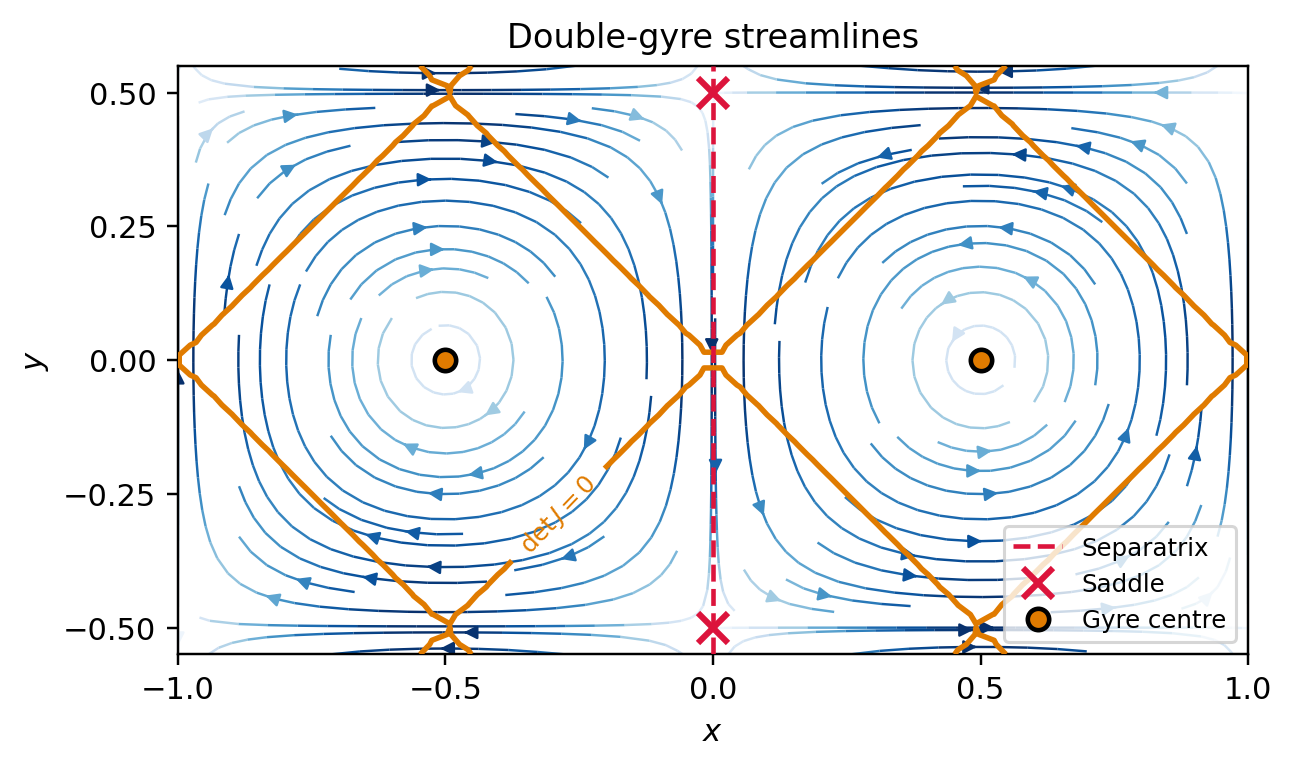
\includegraphics[width=0.45\textwidth]{figures/double_gyre_streamlines.png}
    % TODO: generate with double_gyre_static from
    %   src/fields/environments/Double_Gyre.py.
    % Show: streamlines, separatrix at x=0, saddle points at (0, pm 0.5),
    %   gyre centers at (pm 0.5, 0), det(J)=0 diamonds overlaid.
    \caption{Double-gyre vector field (steady case, $A = 0.1$). Streamlines
    are shown in gray. The separatrix at $x = 0$ (dashed) is the stable
    manifold of the lower saddle and the unstable manifold of the upper
    saddle ($\times$). The $D = 0$ Okubo-Weiss boundary (solid) is a
    diamond around each gyre center ($\bullet$).}
    \label{fig:dg_streamlines}
\end{figure}

\begin{figure}[!t]
    \centering
    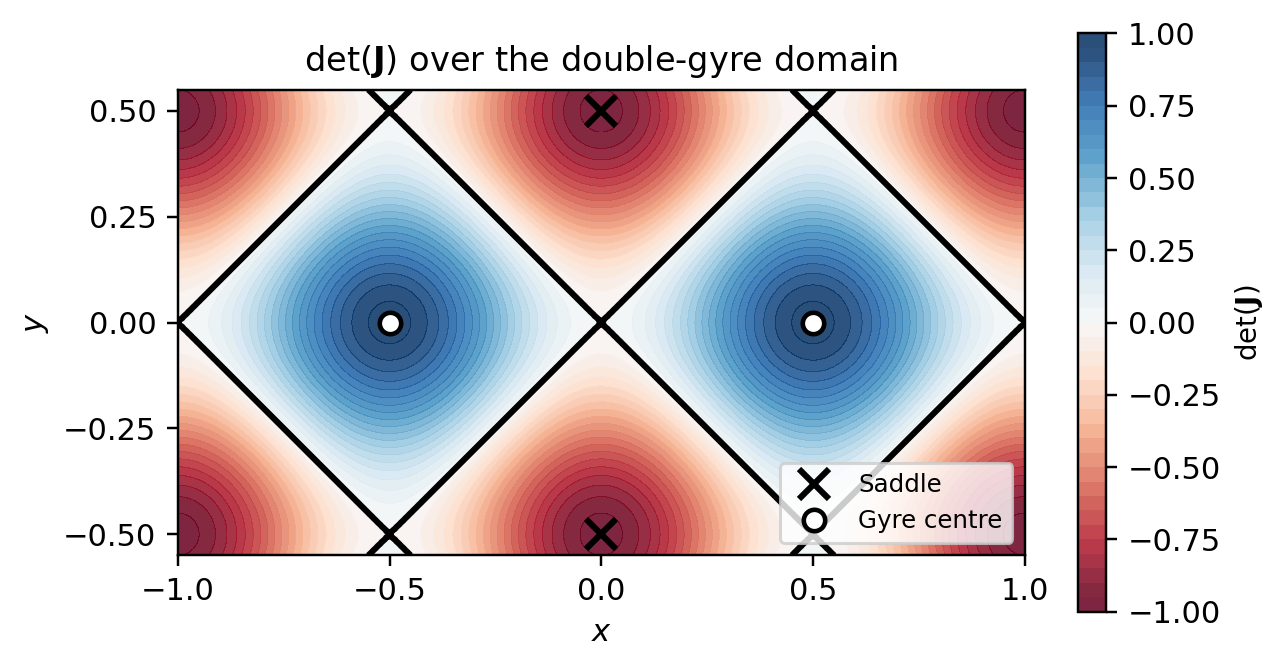
\includegraphics[width=0.45\textwidth]{figures/detJ_contour.png}
    % TODO: contour plot of D from (eq:det_analytic_main). Overlay the zero
    % contour (diamond) in bold; mark saddles, gyre centers, and the trench
    % along x=0.
    \caption{$D = \det(\mathbf{J})$ over the double-gyre domain. The $D = 0$
    boundary (bold) separates rotation-dominated cores ($D > 0$) from the
    strain-dominated exterior ($D < 0$). The separatrix at $x = 0$ is a
    valley line of $D$ connecting the crest at the origin to the two wells
    at the saddle points.}
    \label{fig:detJ_contour}
\end{figure}

\begin{figure}[!t]
    \centering
    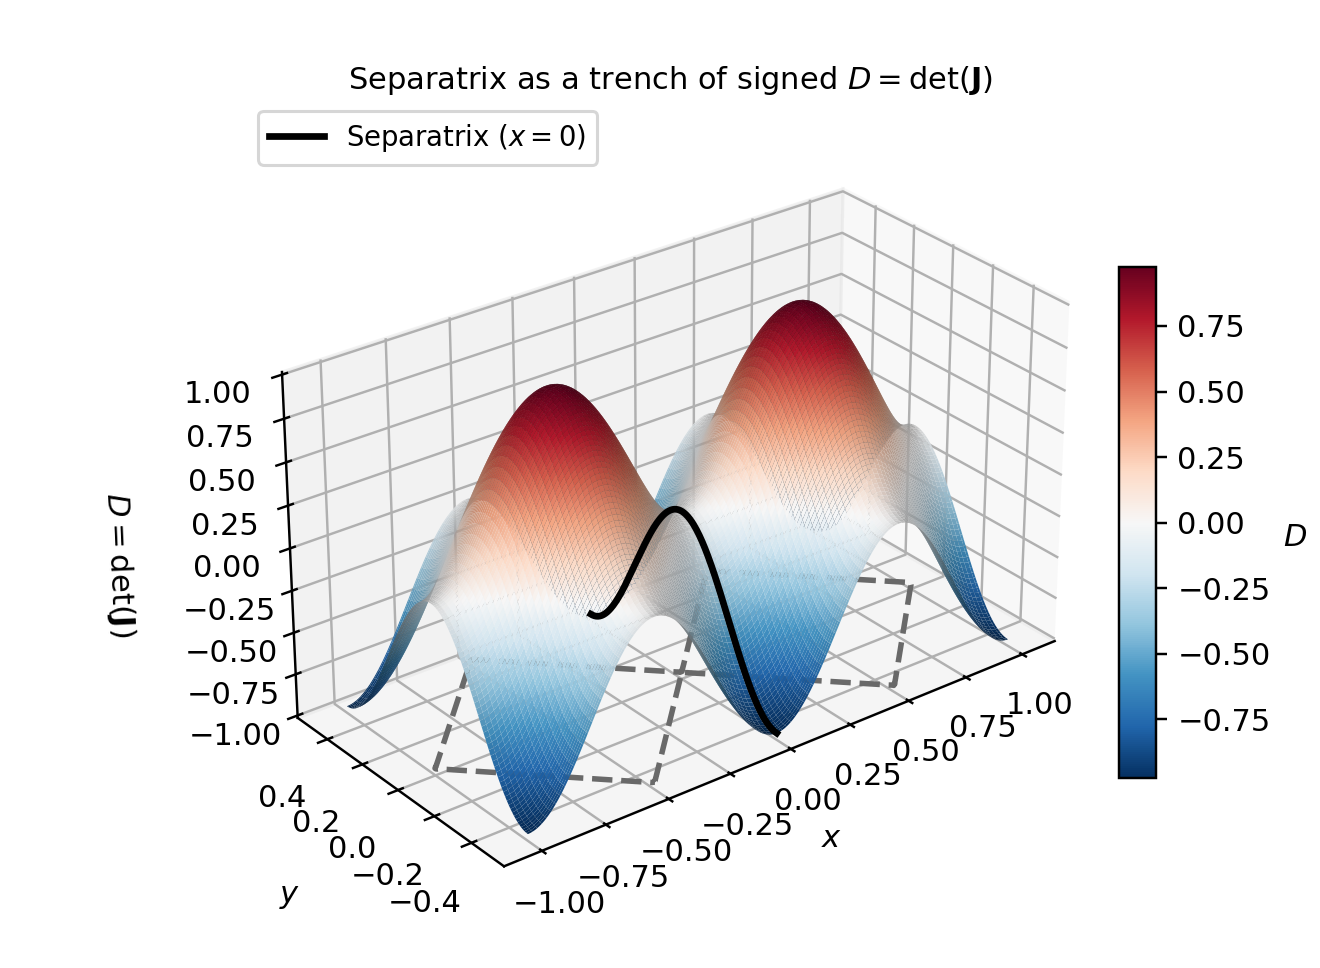
\includegraphics[width=0.45\textwidth]{figures/detJ_trench_cross_section.png}
    % TODO: plot D (signed, not |D|) along horizontal cross-sections at
    % y = 0, 0.2, 0.4 using (eq:det_analytic_main); mark the valley at x=0.
    \caption{$D$ along horizontal cross-sections of the double gyre at
    $y = 0$, $0.2$, and $0.4$. Each section has a local minimum at $x = 0$:
    the separatrix is a trench of the signed field $D$. The trench deepens
    toward the saddle points and its floor rises to $D = 0$ at the origin.}
    \label{fig:trench_cross}
\end{figure}

\subsection{Problem Statement}
\label{sec:problem_statement}

Consider $N$ robots at positions $\mathbf{p}_i$, each measuring the local
flow $(u_i, v_i) = \mathbf{v}(\mathbf{p}_i)$ at the common sampling
instant. No map, forecast, or prior model of the field is available, and
no robot can integrate trajectories of the field. Using only the current
synchronous samples $\{(\mathbf{p}_i, u_i, v_i)\}_{i=1}^{N}$ at each
control cycle, the team must generate a centroid velocity command
$\dot{\mathbf{p}}_c$ that solves:

\emph{Problem 1 (separatrix network traversal).} Drive the cluster
centroid onto the trench of $D$ and travel it, in the direction of the
ambient flow, through the saddle points where trench segments cross.
Terminal capture at a single saddle (Section~\ref{sec:sep_controller}) is
the special case in which the selector's stationary-point test is
tightened to stop the team there instead.

\emph{Problem 2 (Okubo-Weiss boundary tracking).} Drive $D(\mathbf{p}_c)
\to 0$ and travel along the boundary $\mathcal{C}$, a network of the same
kind (Section~\ref{sec:dg_example}).

Both problems require, at minimum, pointwise estimates of $D$, its
gradient $\mathbf{g} = \nabla D$, and its Hessian $\mathbf{H}_D$ at the
centroid. The next section shows how a six-robot formation produces them.


% ---------------------------------------------------------------------------
\section{Distributed Second-Order Estimation}
\label{sec:estimation}

\subsection{Quadratic Fit from Six Simultaneous Measurements}

Let $\tilde{\mathbf{p}}_i = \mathbf{p}_i - \mathbf{p}_c$ denote robot
positions relative to the centroid and define the quadratic basis vector
\begin{equation}
    \boldsymbol{\phi}(\tilde{\mathbf{p}}) =
    \bigl[\,1, \; \tilde{x}, \; \tilde{y}, \; \tfrac{1}{2}\tilde{x}^2, \;
    \tilde{x}\tilde{y}, \; \tfrac{1}{2}\tilde{y}^2\,\bigr]^\top,
    \label{eq:basis}
\end{equation}
whose one-half factors make the fitted coefficients equal to the Taylor
derivatives in (\ref{eq:quad_model_u})--(\ref{eq:quad_model_v}). Stacking
the basis vectors of the six robots row-wise gives the $6 \times 6$
formation matrix $\boldsymbol{\Phi}$, the second-order generalization of
the $3 \times 3$ matrix $\mathbf{A}$ of [6]. The coefficient vectors
$\boldsymbol{\theta}_u = [u_0, u_x, u_y, u_{xx}, u_{xy}, u_{yy}]^\top$ and
$\boldsymbol{\theta}_v = [v_0, v_x, v_y, v_{xx}, v_{xy}, v_{yy}]^\top$
solve the pair of linear systems
\begin{equation}
    \boldsymbol{\Phi}\,\boldsymbol{\theta}_u = \mathbf{u}, \qquad
    \boldsymbol{\Phi}\,\boldsymbol{\theta}_v = \mathbf{v},
    \label{eq:solve}
\end{equation}
where $\mathbf{u} = [u_1, \ldots, u_6]^\top$ and $\mathbf{v} = [v_1,
\ldots, v_6]^\top$ collect the measurements. One matrix factorization
serves both components. When the field is exactly quadratic over the
formation footprint, the solution of (\ref{eq:solve}) is exact for any
nonsingular $\boldsymbol{\Phi}$; for general smooth fields the model
error is quantified in Section~\ref{sec:sensitivity}.

\subsection{Six Robots Are Necessary, and Almost Always Sufficient}

\begin{proposition}[Minimality]
\label{prop:minimality}
Each robot contributes exactly one linear equation to each system in
(\ref{eq:solve}), and each system has six unknowns. Hence no algorithm,
linear or otherwise, can uniquely recover the quadratic model
(\ref{eq:quad_model_u})--(\ref{eq:quad_model_v}) from one synchronous
sample of fewer than six robots, and six robots suffice exactly when
$\boldsymbol{\Phi}$ is nonsingular.
\end{proposition}

\begin{IEEEproof}
With $N < 6$ robots, $\boldsymbol{\Phi} \in \mathbb{R}^{N \times 6}$ has
a nontrivial null space, so for any candidate coefficient vector
$\boldsymbol{\theta}_u$ the vector $\boldsymbol{\theta}_u +
\boldsymbol{\theta}_0$ with $\boldsymbol{\Phi}\boldsymbol{\theta}_0 =
\mathbf{0}$, $\boldsymbol{\theta}_0 \neq \mathbf{0}$, generates identical
measurements at every robot. The two quadratic fields are
indistinguishable from the data, so no estimator can select between
them. With $N = 6$, (\ref{eq:solve}) has a unique solution if and only if
$\det(\boldsymbol{\Phi}) \neq 0$.
\end{IEEEproof}

Nonsingularity has a clean geometric characterization.

\begin{proposition}[Conic criterion]
\label{prop:conic}
$\boldsymbol{\Phi}$ is singular if and only if the six sampling points
lie on a common conic, that is, on the zero set of some nonzero quadratic
polynomial $q(\tilde{x}, \tilde{y})$ (including degenerate conics such as
line pairs).
\end{proposition}

\begin{IEEEproof}
$\boldsymbol{\Phi}$ is singular iff its columns are linearly dependent,
iff there is a nonzero coefficient vector $\mathbf{c}$ with
$\boldsymbol{\phi}(\tilde{\mathbf{p}}_i)^\top \mathbf{c} = 0$ for all
$i$. The function $q = \boldsymbol{\phi}^\top \mathbf{c}$ is precisely a
nonzero polynomial of degree at most two vanishing at all six points.
\end{IEEEproof}

\begin{corollary}[Pentagon plus center]
\label{cor:pentagon}
Place five robots at the vertices of a regular pentagon of radius $\rho$
and the sixth at its center. Then $\boldsymbol{\Phi}$ is nonsingular.
\end{corollary}

\begin{IEEEproof}
No three vertices of a regular pentagon are collinear, and five points in
general position determine a unique conic; for the pentagon vertices that
conic is the circumscribed circle. The center does not lie on the
circle, so no conic passes through all six points, and
Proposition~\ref{prop:conic} applies.
\end{IEEEproof}

\begin{remark}[The center robot is essential]
Any formation whose six robots lie on one circle, for example a regular
hexagon, is singular regardless of its size or orientation, since the
circle itself is a conic through all six points. Rings are natural
formations for mobile robots, which makes this failure mode easy to adopt
by accident; moving one robot to the center removes it entirely.
\end{remark}

\subsection{The Formation and Its Noise Gains}
\label{sec:formation}

The pentagon-plus-center shape is the same minimal configuration that
Bri\~{n}\'{o}n-Arranz et al.\ derived for Hessian estimation of a scalar
field: $N \geq 5$ robots uniformly spaced on a circle plus one at the
center [11]. Their estimator combines the ring measurements with fixed
symmetric weights, which is computationally trivial and, for exactly six
robots on the ideal formation, algebraically equivalent to solving
(\ref{eq:solve}). The two approaches separate when the formation deforms,
as it always does under real formation control: fixed weights assume the
ideal geometry and acquire a bias proportional to the deformation,
whereas (\ref{eq:solve}) uses the measured robot positions and remains
exact for quadratic fields under any deformation short of the conic
degeneracy of Proposition~\ref{prop:conic}. The estimator therefore
degrades gracefully: formation error affects accuracy only through the
conditioning of $\boldsymbol{\Phi}$, which is monitored online through
$\det(\boldsymbol{\Phi})$.

For the ideal formation the noise amplification has closed form. Let each
measurement carry independent zero-mean noise of standard deviation
$\sigma_{uv}$, as in (\ref{eq:meas_noise}). Since
$\hat{\boldsymbol{\theta}}_u - \boldsymbol{\theta}_u =
\boldsymbol{\Phi}^{-1}\boldsymbol{\eta}$, the standard deviation of each
coefficient is $\sigma_{uv}$ times the Euclidean norm of the
corresponding row of $\boldsymbol{\Phi}^{-1}$.

\begin{lemma}[Exact noise gains of the pentagon-plus-center formation]
\label{lem:gains}
For five robots on a ring of radius $\rho$ and one at the centroid, the
coefficient standard deviations are
\begin{equation}
    \sigma_{u_0} = \sigma_{uv}, \quad
    \sigma_{u_x} = \sigma_{u_y} = \frac{2}{\sqrt{10}}\frac{\sigma_{uv}}{\rho},
    \label{eq:gain_grad}
\end{equation}
\begin{equation}
    \sigma_{u_{xx}} = \sigma_{u_{yy}} = \frac{8}{\sqrt{10}}
    \frac{\sigma_{uv}}{\rho^2},
    \qquad
    \sigma_{u_{xy}} = \frac{4}{\sqrt{10}}\frac{\sigma_{uv}}{\rho^2},
    \label{eq:gain_hess}
\end{equation}
independent of the formation heading, and identically for
$\boldsymbol{\theta}_v$.
\end{lemma}

\begin{IEEEproof}
The value coefficient is exact: every basis function except the constant
vanishes at the origin, so interpolation forces $\hat{u}_0$ to equal the
center robot's reading, giving unit gain. The remaining rows follow from
direct inversion of $\boldsymbol{\Phi}$ using the fifth roots of unity;
the row norms reduce to the stated constants, and repeating the
computation with an arbitrary ring phase leaves them unchanged. The
error covariance of the estimated gradient is in fact isotropic,
$\tfrac{4}{10}\sigma_{uv}^2\,\rho^{-2}\mathbf{I}$, for every heading.
\end{IEEEproof}

Two design consequences. First, the gains are isotropic: the error
covariance of the estimated gradient (and of the Hessian, entrywise as
stated) does not depend on the direction of travel, so estimator quality
does not degrade as the cluster turns. Second, the $1/\rho$ and
$1/\rho^2$ factors exhibit the fundamental scaling: second derivatives
are harder to sense than first derivatives by one power of the formation
radius. A numerical search over all six-point formations of the same
footprint found configurations at best a few percent better in worst-case
Hessian gain, so the symmetric shape is used without further tuning.

\begin{figure}[!t]
    \centering
    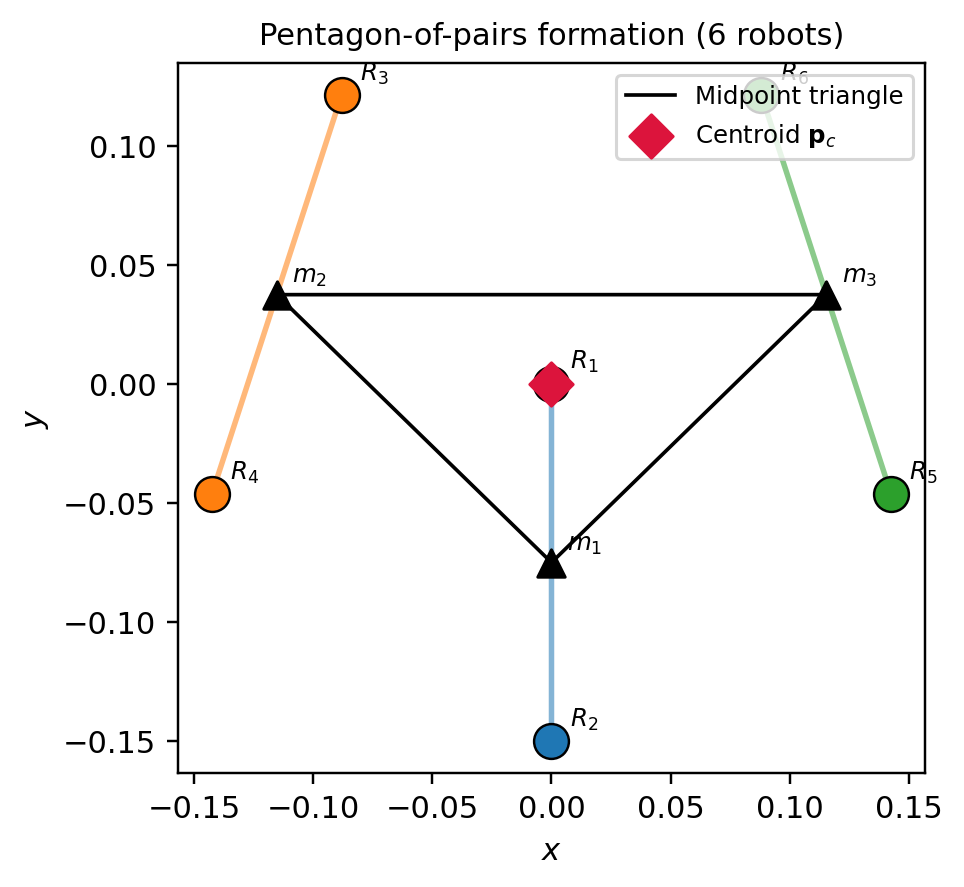
\includegraphics[width=0.40\textwidth]{figures/pentagon_formation.png}
    % TODO: draw the formation: 5 robots on a ring of radius rho at 72 deg
    % spacing, robot 6 at the center. Overlay the three-pair grouping used
    % by the cluster controller (pairs A, B, C with midpoints m1, m2, m3
    % forming the SAS triangle). Annotate rho.
    \caption{Six-robot formation: five robots on a ring of radius $\rho$
    at $72^\circ$ spacing and one robot at the center, the minimal
    symmetric formation for second-order estimation
    (Corollary~\ref{cor:pentagon}, [11]). For formation control the six
    robots are grouped into three pairs whose midpoints define an SAS
    triangle (Appendix~\ref{app:kinematics}); the grouping is invisible to
    the estimator, which uses only the six measured positions.}
    \label{fig:pentagon_formation}
\end{figure}

\subsection{Closed-Form Recovery of $D$, $\nabla D$, and $\mathbf{H}_D$}

The estimated Jacobian at the centroid is assembled from the linear
coefficients,
\begin{equation}
    \hat{\mathbf{J}} =
    \begin{bmatrix} u_x & u_y \\ v_x & v_y \end{bmatrix},
    \qquad
    \hat{D} = u_x v_y - u_y v_x.
    \label{eq:J_hat}
\end{equation}
Under the quadratic model, each entry of $\mathbf{J}$ is an affine
function of position, so $D(\mathbf{p})$ is itself an exactly quadratic
polynomial over the footprint. Its gradient and Hessian at the centroid
are polynomial functions of the fitted coefficients:
\begin{equation}
    \hat{\mathbf{g}} = \nabla \hat{D} =
    \begin{bmatrix}
        u_{xx} v_y + u_x v_{xy} - u_{xy} v_x - u_y v_{xx} \\
        u_{xy} v_y + u_x v_{yy} - u_{yy} v_x - u_y v_{xy}
    \end{bmatrix},
    \label{eq:grad_det}
\end{equation}
\begin{equation}
    \hat{\mathbf{H}}_D =
    \begin{bmatrix}
        2(u_{xx} v_{xy} - u_{xy} v_{xx}) &
        u_{xx} v_{yy} - u_{yy} v_{xx} \\
        u_{xx} v_{yy} - u_{yy} v_{xx} &
        2(u_{xy} v_{yy} - u_{yy} v_{xy})
    \end{bmatrix}.
    \label{eq:hess_det}
\end{equation}
These follow by differentiating $D = u_x v_y - u_y v_x$ with the
third-order terms absent, and require no field evaluations beyond the six
measurements. The omission is harmless for the gradient but not for the
Hessian; its systematic consequences are quantified in
Section~\ref{sec:sensitivity}. The estimated flow at the centroid,
$\mathbf{f} = (u_0, v_0)$, equals the center robot's reading by
Lemma~\ref{lem:gains}. Together
(\ref{eq:J_hat})--(\ref{eq:hess_det}) supply every quantity the
controllers of Section~\ref{sec:controllers} consume: $\hat{D}$,
$\hat{\mathbf{g}}$, $\hat{\mathbf{H}}_D$, and $\mathbf{f}$.

\subsection{Sensitivity: Noise, Truncation, and Formation Radius}
\label{sec:sensitivity}

Three error sources separate cleanly. Write $\boldsymbol{\Phi} =
\bar{\boldsymbol{\Phi}}\,\mathbf{S}_\rho$ with $\mathbf{S}_\rho =
\mathrm{diag}(1, \rho, \rho, \rho^2, \rho^2, \rho^2)$, where
$\bar{\boldsymbol{\Phi}}$ depends only on the formation shape. All
scale dependence enters through $\mathbf{S}_\rho^{-1}$.

\subsubsection{Measurement noise}
By Lemma~\ref{lem:gains}, gradient coefficients degrade as
$\sigma_{uv}/\rho$ and Hessian coefficients as $\sigma_{uv}/\rho^2$:
larger formations average noise better.

\subsubsection{Truncation bias}
If the field is three times differentiable with
$|\partial^3 u|, |\partial^3 v| \leq M_3$ over the footprint, the Taylor
remainder at robot $i$ is bounded by $\tfrac{M_3}{6}\rho^3$, and passing
it through $\mathbf{S}_\rho^{-1}\bar{\boldsymbol{\Phi}}^{-1}$ bounds the
systematic error by
\begin{equation}
    |\hat{u}_x - u_x| \leq c_1 M_3 \rho^2, \qquad
    |\hat{u}_{xx} - u_{xx}| \leq c_2 M_3 \rho,
    \label{eq:truncation}
\end{equation}
and likewise for the remaining coefficients, where $c_1, c_2$ are
absolute constants of the formation shape (row sums of
$|\bar{\boldsymbol{\Phi}}^{-1}|$ divided by six). The Hessian bias decays
only linearly in $\rho$, matching the $O(\rho)$ bound proved for the
symmetric estimator in [11]: smaller formations track curvature better.

\subsubsection{The radius trade-off}
Combining the two effects, the total error of each fitted second-order
coefficient is bounded by
$c_2 M_3 \rho + c_2' \sigma_{uv}/\rho^2$, which is minimized at
\begin{equation}
    \rho^* = \left(\frac{2 c_2' \sigma_{uv}}{c_2 M_3}\right)^{1/3}
    \propto \left(\frac{\sigma_{uv}}{M_3}\right)^{1/3}.
    \label{eq:rho_star}
\end{equation}
The formation radius is thus a sensing parameter, not merely a spacing
choice: it should grow with the noise floor and shrink with the field's
third-derivative scale. This rule is confirmed for $\hat{D}$ and
$\nabla\hat{D}$ by the formation-radius sweeps reported in
Section~\ref{sec:results}; the derived Hessian $\hat{\mathbf{H}}_D$ is
instead limited by the model bias discussed next.

\subsubsection{Propagation to $D$ and its derivatives}
Errors in the fitted coefficients enter the navigation quantities through
products of coefficient pairs. For two-by-two matrices the expansion of
the determinant is exact at second order:
$\det(\mathbf{J} + \mathbf{E}) = \det(\mathbf{J}) +
\operatorname{tr}(\mathrm{adj}(\mathbf{J})\mathbf{E}) + \det(\mathbf{E})$,
and $\|\mathrm{adj}(\mathbf{J})\|_F = \|\mathbf{J}\|_F$, so the estimated
determinant satisfies
\begin{equation}
    |\hat{D} - D| \;\leq\; \|\mathbf{J}\|_F \|\mathbf{E}\|_F
    + \tfrac{1}{2}\|\mathbf{E}\|_F^2,
    \label{eq:det_perturbation}
\end{equation}
where $\mathbf{E} = \hat{\mathbf{J}} - \mathbf{J}$ collects the four
first-order coefficient errors. The gradient formula (\ref{eq:grad_det})
is complete: differentiating $D = u_x v_y - u_y v_x$ once produces only
products of first- and second-order derivatives, so $\hat{\mathbf{g}}$
inherits errors solely from the fitted coefficients, linearly, with
slopes set by the true derivative magnitudes.

The Hessian is different in kind. Differentiating twice produces terms
such as $u_{xxx} v_y$ and $u_y v_{xxx}$, third derivatives of the field
weighted by the field itself, and a quadratic model has no third
derivatives: (\ref{eq:hess_det}) is the Hessian of the fitted quadratic
surface, not of $D$. The omitted terms constitute a model bias that is
independent of the formation radius and cannot be reduced by averaging;
the situation is that of fitting a line to a curved signal and using the
line's slope where the curvature is unmodeled, acceptable exactly where
the model is locally adequate. For the double gyre at the nominal scale
this bias is large in norm, on the order of $\|\mathbf{H}_D\|_F$ itself
(Section~\ref{sec:results}). Two conclusions nevertheless carry into the
stability analysis: the estimate errors entering the controllers are
bounded whenever the coefficient errors are bounded, with explicit
formation-dependent constants; and all such constants degrade
continuously, not abruptly, as the formation deforms, with outright
failure only on the conic configurations of
Proposition~\ref{prop:conic}.

\begin{remark}[What survives the Hessian bias]
\label{rem:eigvec}
The controllers of Section~\ref{sec:controllers} consume
$\hat{\mathbf{H}}_D$ only through its eigenvectors and the signs and
rough magnitudes of its eigenvalues, and these degrade far less than the
Frobenius error suggests. The double gyre is symmetric under reflection
across the separatrix, so $D$ is even in the transverse coordinate and
every odd transverse derivative, including the mixed second derivative,
vanishes on the trench: both the retained and the omitted terms are
diagonal in the trench frame there. The estimated eigen-directions on
the separatrix are exact to numerical precision, remain within a few
tenths of a degree across the tube, and within a few degrees at generic
points (Section~\ref{sec:results}), while the bias loads almost entirely
onto the eigenvalues. The transverse Newton snap divides the transverse
gradient by the transverse eigenvalue, so an eigenvalue bias rescales
the step, which the saturation (\ref{eq:sat}) bounds and the closed loop
absorbs; it does not rotate the commanded direction. This is why a
formation too small to sense curvature accurately can still track the
structure that curvature defines. The exception is the immediate
neighborhood of the wells, where the biased eigenvalues nearly vanish
and their signs become unreliable; the consequences for terminal capture
are examined in Section~\ref{sec:results}.
\end{remark}


% ---------------------------------------------------------------------------
\section{Adaptive Navigation Controllers}
\label{sec:controllers}

\subsection{Control Architecture}
\label{sec:arch}

Both controllers run inside the three-layer architecture of [6, 12]:

\begin{enumerate}
    \item \textbf{Navigation primitive.} From the six positions and
          measurements, compute the estimates
          (\ref{eq:J_hat})--(\ref{eq:hess_det}) and output a centroid
          velocity command $\dot{\mathbf{p}}_c^{\,\text{des}}$. The two
          primitives of this section differ only in this block.
    \item \textbf{Cluster space controller.} Using the twelve-state
          cluster parameterization and its analytic inverse kinematic
          Jacobian (Appendix~\ref{app:kinematics}), distribute the
          centroid command to six robot velocity commands while
          regulating the formation shape to its nominal geometry.
    \item \textbf{Robot dynamics.} Each robot obeys the first-order
          momentum model identified on the Decabot hardware [6],
          \begin{equation}
              \mathbf{v}[k+1] = \alpha_{\text{mom}}\,\mathbf{v}[k]
              + (1 - \alpha_{\text{mom}})\,\mathbf{v}^{\text{des}}[k],
              \label{eq:momentum}
          \end{equation}
          with $\alpha_{\text{mom}} = \exp(-\Delta t/\tau)$, actuator
          time constant $\tau = 0.3$ s, control period $\Delta t = 0.1$ s
          (so $\alpha_{\text{mom}} \approx 0.717$), speed limit
          $v_{\text{max,robot}} = 0.3$ m/s, and stiction floor
          $v_{\text{stiction}} = 0.025$ m/s.
          % 0.05 m/s was the three-robot paper's value; the six-robot
          % simulation uses the Omnibot default 0.025 (omnibot.py).
\end{enumerate}

Note on notation: $\alpha_{\text{mom}}$ in (\ref{eq:momentum}) is the
momentum coefficient of the robot model; it is unrelated to
$\alpha_{\text{eig}}$, the real part of a complex eigenvalue pair of
$\mathbf{J}$ used in field classification.

\subsection{From the Newton Step to the Modified Newton Step}
\label{sec:mod_newton}

Under the quadratic model, $\hat{D}(\mathbf{p})$ is an exact quadratic
surface with gradient $\hat{\mathbf{g}}$ and constant Hessian
$\hat{\mathbf{H}}_D$ at the centroid, so the natural navigation move is
the Newton step $\Delta\mathbf{p} = -\hat{\mathbf{H}}_D^{-1}
\hat{\mathbf{g}}$, which jumps to the stationary point of the local
model in one move. Written in the eigenbasis
$\hat{\mathbf{H}}_D \mathbf{w}_k = \lambda_k \mathbf{w}_k$, with
$\lambda_1 \leq \lambda_2$ throughout, the step decomposes into
per-direction components $-(\mathbf{w}_k^\top
\hat{\mathbf{g}})/\lambda_k$. Two defects make the raw step unsuitable
as a velocity command, and each is repaired by one modification.

First, the magnitude is unbounded and explodes where
$\hat{\mathbf{H}}_D$ is near singular. The repair is componentwise
saturation through
\begin{equation}
    \mathrm{sat}(c) = v_{\max} \tanh\!\left(\frac{c}{v_{\max}}\right),
    \label{eq:sat}
\end{equation}
which gives a bounded constant-speed reach far from the structure and
recovers the exact Newton component, with its superlinear local
convergence, once $|c| \ll v_{\max}$. A single parameter $v_{\max}$
sets both the cruise speed and the width of the terminal boundary
layer. The saturated Newton step is the \emph{attract step},
\begin{equation}
    \dot{\mathbf{p}}_c^{\,\text{des}} = \sum_{k=1}^{2}
    \mathrm{sat}\!\left(-\frac{\mathbf{w}_k^\top
    \hat{\mathbf{g}}}{\lambda_k}\right)\mathbf{w}_k.
    \label{eq:attract_step}
\end{equation}

Second, and more fundamentally, (\ref{eq:attract_step}) converges to
whatever stationary point the local model exhibits, with no preference
among minima, maxima, and saddle points of $D$. On a trench the
along-trench curvature can be negative (the crest side), and there the
Newton component deliberately climbs. The modification, adopted from
saddle-free Newton methods in optimization [18], replaces the signed
eigenvalue by its magnitude, giving the \emph{slide step},
\begin{equation}
    \dot{\mathbf{p}}_c^{\,\text{des}} = \sum_{k=1}^{2}
    \mathrm{sat}\!\left(-\frac{\mathbf{w}_k^\top
    \hat{\mathbf{g}}}{|\lambda_k|}\right)\mathbf{w}_k.
    \label{eq:slide_step}
\end{equation}
In directions of positive curvature the two laws agree and snap the
centroid onto the trench floor; in the direction of negative curvature
(\ref{eq:slide_step}) reverses the Newton component into a
curvature-normalized descent that slides along the trench, away from
crests. Both laws are well defined despite the sign ambiguity of
eigenvectors: every term is quadratic in $\mathbf{w}_k$, so replacing
$\mathbf{w}_k$ by $-\mathbf{w}_k$ leaves the command unchanged.

\subsection{Controller 1: Separatrix Tracker}
\label{sec:sep_controller}

The separatrix tracker composes the two step bodies with a third,
flow-assisted mode. The need for the third mode is visible in the trench
profile of Section~\ref{sec:dg_example}: the slide step descends $D$
along the trench, but at the crest the along-trench gradient vanishes,
and on the upstream side of the crest descent points away from the flow
direction, while the separatrix continues through the crest. On the
separatrix itself, however, the ambient flow is tangent to the structure
and nonzero away from the saddles, so the flow can carry the team across
the crest. The cluster is declared on the separatrix
(FLOW band) when either
\begin{equation}
    |\hat{D}| < \varepsilon_{\text{raw}}
    \quad\text{or}\quad
    \frac{|\hat{D}|}{\|\hat{\mathbf{H}}_D\|_F} < \varepsilon_{\text{dim}},
    \label{eq:flow_band}
\end{equation}
where $\varepsilon_{\text{raw}}$ is a raw threshold and
$\varepsilon_{\text{dim}}$ a curvature-normalized threshold (units of
length squared) that makes the band scale with the local landscape. In
the FLOW band the command follows the measured flow along the trench
tangent $\mathbf{w}_1$ and retains the Newton snap across it: the
\emph{flow step} is
\begin{equation}
    \dot{\mathbf{p}}_c^{\,\text{des}} =
    \mathrm{sat}\!\left(\mathbf{f}^\top \mathbf{w}_1\right)\mathbf{w}_1
    + \mathrm{sat}\!\left(-\frac{\hat{\mathbf{g}}^\top
    \mathbf{w}_2}{\lambda_2}\right)\mathbf{w}_2.
    \label{eq:flow_step}
\end{equation}
Off the band, the local flow direction selects between the attract and
slide laws: if the flow agrees with the along-trench descent direction
the team slides (\ref{eq:slide_step}); if it opposes descent the team
attracts toward the local stationary point (\ref{eq:attract_step}),
which lies at the crest, inside the FLOW band, so the attract law hands
the team over to the flow. In all three modes the tangential motion is
never directed against the ambient flow, a fact used in the stability
analysis. The complete selector, executed once per control cycle after
the estimation step, is:

\vspace{4pt}
\hrule
\vspace{4pt}
\noindent\textbf{Separatrix tracker: one control cycle}

\vspace{3pt}
\noindent\textbf{Parameters:} $v_{\max}$, $\varepsilon_{\text{raw}}$,
$\varepsilon_{\text{dim}}$\\
\textbf{Given:} $\hat{D}$, $\hat{\mathbf{g}}$, $\hat{\mathbf{H}}_D$,
$\mathbf{f}$ from (\ref{eq:J_hat})--(\ref{eq:hess_det}), and eigenpairs
$(\lambda_1, \mathbf{w}_1)$, $(\lambda_2, \mathbf{w}_2)$ of
$\hat{\mathbf{H}}_D$, $\lambda_1 \leq \lambda_2$

\vspace{3pt}
\noindent If the band test (\ref{eq:flow_band}) passes (on the
separatrix):\\
\hspace*{1.5em} apply the flow step (\ref{eq:flow_step}).\\
Else, if $\lambda_1 \lambda_2 \geq 0$ ($\hat{D}$ has no saddle; near a
well of $D$):\\
\hspace*{1.5em} apply the attract step (\ref{eq:attract_step}).\\
Else, orient $\mathbf{w}_1$ so that $\hat{\mathbf{g}}^\top \mathbf{w}_1
\leq 0$ (descent along the trench):\\
\hspace*{1.5em} if $\mathbf{f}^\top \mathbf{w}_1 > 0$ (flow agrees with
descent), apply the slide step (\ref{eq:slide_step});\\
\hspace*{1.5em} otherwise (flow opposes descent), apply the attract
step (\ref{eq:attract_step}).
\vspace{4pt}
\hrule
\vspace{4pt}

The implementation is \textit{separatrix\_logic\_c\_step} in
\textit{pentagon\_primitives.py}. Note that the $\mathbf{w}_2$
component is one and the same in all three laws
(\ref{eq:attract_step}), (\ref{eq:slide_step}), and
(\ref{eq:flow_step}): on a trench, $\lambda_2 > 0$, so the signed and
magnitude denominators agree, and every mode applies the identical
transverse Newton snap. The modes differ only in their motion along the
structure. This shared component is what makes the switched system
tractable in Section~\ref{sec:stability}.

\subsection{Controller 2: Okubo-Weiss Boundary Tracker}
\label{sec:ow_controller}

The boundary tracker solves Problem 2: drive the scalar $\hat{D}$ to
zero and travel along the level set $\mathcal{C}$. Its transverse
action is a Newton step for the scalar root-finding problem
$D(\mathbf{p}) = 0$: the displacement
$-(\hat{D}/\|\hat{\mathbf{g}}\|^2)\,\hat{\mathbf{g}}$ is the smallest
step that zeroes the linearized $D$, and its length
$|\hat{D}|/\|\hat{\mathbf{g}}\|$ is the estimated distance to the
boundary. Its tangential action drifts along the tangent of the level
set, which is perpendicular to the gradient by definition. With the
unit vectors
\begin{equation}
    \hat{\mathbf{u}} = -\mathrm{sign}(\hat{D})\,
    \frac{\hat{\mathbf{g}}}{\|\hat{\mathbf{g}}\|},
    \qquad
    \hat{\mathbf{t}} = \pm\,\mathbf{R}_{90^\circ}
    \frac{\hat{\mathbf{g}}}{\|\hat{\mathbf{g}}\|},
    \label{eq:ow_directions}
\end{equation}
where $\mathbf{R}_{90^\circ}$ is the quarter-turn rotation and the sign
of $\hat{\mathbf{t}}$ is chosen so that $\mathbf{f}^\top
\hat{\mathbf{t}} \geq 0$ (the team circulates with the flow), the
control law is
\begin{equation}
    \dot{\mathbf{p}}_c^{\,\text{des}} =
    \mathrm{sat}\!\left(\frac{|\hat{D}|}{\|\hat{\mathbf{g}}\|}\right)
    \hat{\mathbf{u}}
    + \mathrm{sat}\!\left(\mathbf{f}^\top \hat{\mathbf{t}}\right)
    \hat{\mathbf{t}}.
    \label{eq:ow_law}
\end{equation}
This has the same radial-plus-tangential structure as the orbital
controller of [6], with the estimated boundary distance playing the
role of the radial error. When $\|\hat{\mathbf{g}}\| <
\varepsilon_{\text{grad}}$ the directions (\ref{eq:ow_directions}) are
undefined and the law falls back to drifting with the flow,
$\dot{\mathbf{p}}_c^{\,\text{des}} = \mathrm{sat}(\|\mathbf{f}\|)\,
\mathbf{f}/\|\mathbf{f}\|$; Section~\ref{sec:stab_ow} shows this
fallback is needed only at isolated points of $\mathcal{C}$. The
implementation is \textit{logic\_g\_newton\_contour\_pentagon} in
\textit{pentagon\_primitives.py}.

\subsection{Gains and Velocity Limits}

Both controllers saturate every component through $v_{\max}\tanh(c /
v_{\max})$, so the commanded centroid speed never exceeds
$\sqrt{2}\,v_{\max}$. The primitive-level saturation speed is $v_{\max}
= 0.04$ m/s, amplified by a fixed navigation gain $k = 3$ before the
cluster layer so that steady commands clear the robots' stiction floor;
the robot-level limits of (\ref{eq:momentum}) are unchanged from [6].
The band thresholds $\varepsilon_{\text{raw}} = 10^{-3}$ and
$\varepsilon_{\text{dim}} = 0.025$ and the gradient floor
$\varepsilon_{\text{grad}} = 10^{-6}$ are fixed in all experiments
unless noted.

Table~\ref{tab:params} collects the values used in all experiments.

\begin{table}[!t]
\centering
\caption{Simulation and controller parameters}
\label{tab:params}
\footnotesize
\setlength{\tabcolsep}{4pt}
\begin{tabular}{llll}
\hline
\textbf{Symbol} & \textbf{Value} & \textbf{Units} & \textbf{Description} \\
\hline
$v_{\max}$ & 0.04 & m/s & primitive saturation speed \\
$k$ & 3.0 & -- & navigation gain \\
$v_{\text{max,robot}}$ & 0.3 & m/s & robot speed limit \\
$v_{\text{stiction}}$ & 0.025 & m/s & robot stiction floor \\
$\tau$ & 0.3 & s & actuator time constant \\
$\Delta t$ & 0.1 & s & control period \\
$\alpha_{\text{mom}}$ & 0.717 & -- & momentum coefficient $e^{-\Delta t/\tau}$ \\
$A$ & 0.1 & -- & double-gyre amplitude \\
$\rho$ & 0.075 & m & formation ring radius \\
$\varepsilon_{\text{raw}}$ & $10^{-3}$ & s$^{-2}$ & FLOW-band raw threshold \\
$\varepsilon_{\text{dim}}$ & 0.025 & m$^{2}$ & FLOW-band dimensionless threshold \\
$\varepsilon_{\text{grad}}$ & $10^{-6}$ & s$^{-2}$m$^{-1}$ & gradient floor (OW law) \\
\hline
\end{tabular}
\end{table}


% ---------------------------------------------------------------------------
\section{Stability Analysis}
\label{sec:stability}

\subsection{Closed-Loop Model and Standing Assumptions}

The analysis is carried out at the navigation level: the cluster
centroid is modeled as a kinematic integrator
\begin{equation}
    \dot{\mathbf{p}}_c = k\,\boldsymbol{\delta}(\mathbf{p}_c),
    \label{eq:kinematic_model}
\end{equation}
where $\boldsymbol{\delta}$ is the output of the separatrix tracker or
of the boundary-tracking law (\ref{eq:ow_law}), and $k > 0$ is the
navigation gain. This abstracts the cluster and robot layers, whose
tracking dynamics (\ref{eq:momentum}) are faster than the navigation
timescale ($\tau = 0.3$ s against transit times of tens of seconds);
the same separation was validated in hardware in [6]. Time is rescaled
so that $k = 1$. Unless stated otherwise the estimates are taken exact
($\hat{D} = D$, $\hat{\mathbf{g}} = \mathbf{g}$, $\hat{\mathbf{H}}_D =
\mathbf{H}_D$, $\mathbf{f} = \mathbf{v}(\mathbf{p}_c)$);
Section~\ref{sec:stab_iss} restores bounded estimation error.
Throughout, $\mathbf{w}_1, \mathbf{w}_2$ denote unit eigenvectors of
$\mathbf{H}_D$ with $\lambda_1 \leq \lambda_2$, and $z_k =
(\mathbf{w}_k^\top \mathbf{g})/\lambda_k$ the Newton components, so
that the attract step (\ref{eq:attract_step}) reads
$\boldsymbol{\delta} = -\sum_k \mathrm{sat}(z_k)\,\mathbf{w}_k$.

\subsection{The Attract Mode Is a Gradient-Norm Descent}

The first result needs no trench structure at all: it certifies the attract step
globally, wherever $\mathbf{H}_D$ is nonsingular.

\begin{theorem}[Attract-mode certificate]
\label{thm:attract}
Let $V_A = \tfrac{1}{2}\|\mathbf{g}(\mathbf{p}_c)\|^2$. Along
(\ref{eq:kinematic_model}) with the attract step
(\ref{eq:attract_step}),
\begin{equation}
    \dot{V}_A = -v_{\max} \sum_{k=1}^{2} \lambda_k^2\,
    z_k \tanh\!\left(\frac{z_k}{v_{\max}}\right) \;\leq\; 0,
    \label{eq:VA_dot}
\end{equation}
with equality exactly where $\mathbf{g} = \mathbf{0}$. Consequently
every bounded trajectory on which $\mathbf{H}_D$ remains nonsingular
converges to the critical set $\{\mathbf{g} = \mathbf{0}\}$ of $D$, and
isolated critical points with $\mathbf{H}_D$ nonsingular are locally
exponentially stable.
\end{theorem}

\begin{IEEEproof}
Since $\nabla V_A = \mathbf{H}_D \mathbf{g}$,
$\dot{V}_A = \mathbf{g}^\top \mathbf{H}_D \boldsymbol{\delta}
= -\sum_k v_{\max} \tanh(z_k/v_{\max})\,
\mathbf{g}^\top \mathbf{H}_D \mathbf{w}_k
= -\sum_k v_{\max} \tanh(z_k/v_{\max})\,\lambda_k
(\mathbf{w}_k^\top\mathbf{g})$, and $\lambda_k(\mathbf{w}_k^\top
\mathbf{g}) = \lambda_k^2 z_k$, giving (\ref{eq:VA_dot}); each summand
is nonnegative because $z\tanh z \geq 0$. Equality requires $z_1 = z_2 =
0$, that is $\mathbf{g} = \mathbf{0}$. Convergence to the critical set
follows from the invariance principle. Near an isolated critical point
$|z_k| \ll v_{\max}$, the saturation is inactive at first order,
$\boldsymbol{\delta} \approx -\mathbf{H}_D^{-1}\mathbf{g} \approx
-(\mathbf{p}_c - \mathbf{p}^\star_D)$, a unit-rate linear contraction.
\end{IEEEproof}

Theorem~\ref{thm:attract} explains the two roles the attract step plays
in the selector. Far from the trench it provides the approach: it descends
$\|\nabla D\|^2$ toward the stationary set of $D$, which for the double
gyre consists of the trench line's crest and wells and the gyre
centers. Near a well of $D$, where $\mathbf{H}_D \succ 0$, it is the
terminal capture law: the well is the saddle point of the flow, and
convergence is exponential.

\subsection{Separatrix Tracker}
\label{sec:stab_sep}

The trench is formalized as a valley line. The double gyre satisfies all
of the following exactly, with the constants given below.

\begin{assumption}[Nondegenerate straight trench]
\label{ass:trench}
There is a segment $\Gamma$ (take it along the unit vector
$\hat{\mathbf{e}}_\parallel$, with normal $\hat{\mathbf{e}}_\perp$, and
coordinates $(s, n)$) and a tube $T_w = \{|n| \leq w\}$ on which
\begin{equation}
    D(s, n) = \varphi(s) + \tfrac{1}{2}\lambda_\perp(s)\,n^2,
    \qquad 0 < \underline{\lambda} \leq \lambda_\perp(s),
    \label{eq:normal_form}
\end{equation}
the cross terms vanish
($\hat{\mathbf{e}}_\perp^\top \mathbf{H}_D \hat{\mathbf{e}}_\parallel
= 0$ on $T_w$), and on $T_w$ the eigenvalue gap satisfies
$\lambda_2 - \lambda_1 \geq \gamma > 0$ wherever the selector is
outside its attract fallback. For the double gyre separatrix,
(\ref{eq:normal_form}) holds with $n = x$, $s = y$, $\varphi(s) =
-\tfrac{\pi^4 A^2}{2}(1 + \cos 2\pi s_f)$ exactly (the field
(\ref{eq:det_analytic_main}) is additively separable), and
$\lambda_\perp = 2\pi^6 A^2 \cos 2\pi x_f \geq \underline{\lambda}$ on
any tube with $w < 1/4$.
\end{assumption}

\begin{assumption}[Flow structure on the trench]
\label{ass:flow}
$\Gamma$ is an invariant curve of the flow: $\mathbf{v}$ restricted to
$\Gamma$ is tangent to it, with $\|\mathbf{v}\| \geq f_{\min} > 0$
outside balls of radius $r_0$ around the flow saddles, where the flow
vanishes. Along $\Gamma$, the stationary points of $\varphi$ are of two
kinds only: wells located at the flow saddles, and crests located inside
the FLOW band (\ref{eq:flow_band}); quantitatively, $|\varphi'(s)| \geq
m_\varphi > 0$ wherever the band condition fails on $\Gamma$.
\end{assumption}

\begin{lemma}[Common transverse contraction]
\label{lem:transverse}
Under Assumption~\ref{ass:trench}, in every mode of the separatrix
tracker the transverse coordinate obeys
\begin{equation}
    \dot{n} = -v_{\max}\tanh\!\left(\frac{n}{v_{\max}}\right),
    \label{eq:n_dynamics}
\end{equation}
so $|n|$ decreases strictly for $n \neq 0$, the tube $T_w$ is forward
invariant, and $n \to 0$ exponentially once $|n| \leq v_{\max}$. In
particular (\ref{eq:n_dynamics}) is unaffected by arbitrary switching
among the three modes.
\end{lemma}

\begin{IEEEproof}
By (\ref{eq:normal_form}) the Hessian is diagonal in
$(\hat{\mathbf{e}}_\parallel, \hat{\mathbf{e}}_\perp)$ with transverse
eigenvalue $\lambda_\perp > 0$ and eigenvector
$\hat{\mathbf{e}}_\perp$, and the transverse gradient component is
$\hat{\mathbf{e}}_\perp^\top \mathbf{g} = \lambda_\perp n$. The
$\hat{\mathbf{e}}_\perp$ component of the attract step
(\ref{eq:attract_step}), of the slide step (\ref{eq:slide_step}) (the
transverse eigenvalue is positive, so the signed and magnitude
denominators agree), and of the flow step (\ref{eq:flow_step}) are all
built from the same argument $-\lambda_\perp n / \lambda_\perp = -n$.
Saturation gives (\ref{eq:n_dynamics}). The right side is negative for $n > 0$ and
positive for $n < 0$, so $V_\perp = \tfrac{1}{2}n^2$ is a common
Lyapunov function for the switched system; for $|n| \leq v_{\max}$,
$\tanh(n/v_{\max}) \geq n \tanh(1)/v_{\max}$ yields $\dot{V}_\perp \leq
-2\tanh(1) V_\perp$.
\end{IEEEproof}

\begin{lemma}[Flow-consistent progress]
\label{lem:progress}
Under Assumptions~\ref{ass:trench} and \ref{ass:flow}, on $\Gamma$
(after the transient of Lemma~\ref{lem:transverse}) the tangential
velocity component $\dot{s}$ satisfies, in every mode,
$\dot{s}\,(\mathbf{v}^\top \hat{\mathbf{e}}_\parallel) \geq 0$: the team
never moves against the ambient flow along the trench. Moreover
$|\dot{s}| \geq m > 0$ outside the $r_0$ balls, with
\begin{equation}
    m = \min\Bigl\{
    v_{\max}\tanh\!\bigl(\tfrac{f_{\min}}{v_{\max}}\bigr),\;
    v_{\max}\tanh\!\bigl(\tfrac{m_\varphi}
    {\bar{\lambda}_\parallel v_{\max}}\bigr)
    \Bigr\},
    \label{eq:progress_rate}
\end{equation}
where $\bar{\lambda}_\parallel$ bounds $|\lambda_1|$ on the tube.
\end{lemma}

\begin{IEEEproof}
On $\Gamma$ the tangential gradient component is $\varphi'(s)$ and the
along-trench eigenvector is $\hat{\mathbf{e}}_\parallel$. In the FLOW band
the tangential command is $v_{\max}\tanh((\mathbf{f}^\top
\mathbf{w}_1)/v_{\max})$ applied along $\mathbf{w}_1 = \pm
\hat{\mathbf{e}}_\parallel$; the product form makes it a nonnegative
multiple of the flow's tangential component, and by
Assumption~\ref{ass:flow} the crest region is covered by this mode, with
magnitude at least the first argument of (\ref{eq:progress_rate}). Off
the band, the slide step is selected precisely when the flow agrees with the
descent direction $-\mathrm{sign}(\varphi')\hat{\mathbf{e}}_\parallel$,
and its tangential command moves along descent with magnitude
$v_{\max}\tanh(|\varphi'|/(|\lambda_1| v_{\max}))$; the attract step is selected
when the flow opposes descent, and its tangential command,
$-\varphi'/\lambda_1$ with $\lambda_1 < 0$, moves along ascent, which by
the selector's own condition is again the flow direction, with the same
magnitude. In the attract fallback ($\mathbf{H}_D \succeq 0$ near the
wells) the tangential command descends toward the well, which is the
flow direction near a stable-manifold endpoint. In all cases the sign
agrees with the flow and the magnitude is bounded below by
(\ref{eq:progress_rate}) via Assumption~\ref{ass:flow}.
\end{IEEEproof}

\begin{theorem}[Separatrix network traversal]
\label{thm:separatrix}
Under Assumptions~\ref{ass:trench} and \ref{ass:flow}, with exact
estimates, every trajectory of the separatrix tracker starting in the
tube $T_w$
(i) remains in $T_w$ and converges exponentially to the trench, and (ii)
traverses the trench in the direction of the ambient flow, reaching the
$r_0$ neighborhood of a flow saddle in finite time bounded by
$L_\Gamma/m$ with $L_\Gamma$ the trench length. At the saddle, $D$
attains a local minimum with $\mathbf{H}_D \succ 0$
($\mathbf{H}_D = 2\pi^6 A^2\,\mathbf{I}$ at the double-gyre saddles), so
the selector's stationary-point test $\lambda_1\lambda_2 \geq 0$
(Section~\ref{sec:sep_controller}) is satisfied there and (iii)
Theorem~\ref{thm:attract} gives local exponential convergence to the
saddle, terminal capture, exactly as stated. The trench, however, is not
a single arc: Section~\ref{sec:dg_example} shows the saddle is a
crossing of two trench segments running perpendicular to one another. A
selector that reaches the ball and does not satisfy the stationary-point
test, because its estimate of $\mathbf{H}_D$ fails to certify positive
definiteness there, remains in the FLOW or SLIDE modes of
Assumption~\ref{ass:flow} and continues onto the crossing segment
instead of capturing, repeating (i)-(ii) with $\Gamma$ now the new
segment. Capture and continuation are the same theorem applied to
different premises at the crossing; which one the physical controller
exhibits is an estimation question, addressed next.
\end{theorem}

\begin{IEEEproof}
(i) is Lemma~\ref{lem:transverse}. (ii): by Lemma~\ref{lem:progress},
$s(t)$ is monotone in the flow direction with rate at least $m$ outside
the $r_0$ balls, and mode switches cannot reverse it, so the ball is
reached in time at most $L_\Gamma/m$. Capture (iii): inside the ball,
$\mathbf{H}_D \succ 0$, the selector is in its attract fallback, and
Theorem~\ref{thm:attract} gives local exponential convergence to the
well, which coincides with the flow saddle $\mathbf{p}^*$. Continuation:
if the fallback test fails to trigger despite $\mathbf{H}_D \succ 0$
holding for the true field, the selector instead falls through to
Lemma~\ref{lem:progress}'s flow or descent case on whichever of the two
crossing segments the flow direction and sign convention of
$\hat{\mathbf{g}}$ select, and (i)-(ii) apply unchanged with $\Gamma$
relabeled.
\end{IEEEproof}

\begin{remark}[Role of each mode]
The proof assigns each mode a precise job: the transverse Newton snap
(common to all modes) makes the trench attractive; the slide step produces the
descent along the trench; the flow step carries the team across the crest, where
descent is undefined; the attract step turns upstream starts around by climbing to
the crest, and, when its stationary-point test fires at a well, doubles as the
terminal capture law. The
hybrid has no chattering issue in the transverse channel because all
modes share the dynamics (\ref{eq:n_dynamics}).
\end{remark}

\begin{remark}[Capture depends on an estimated, not exact, Hessian]
\label{rem:capture_gap}
Theorem~\ref{thm:separatrix} is stated for exact estimates, under which
$\mathbf{H}_D \succ 0$ at the saddle is certified and capture occurs.
Remark~\ref{rem:eigvec} identifies exactly where this fails for the
closed-form estimator: near the wells the biased eigenvalues nearly
vanish and their signs become unreliable, so the stationary-point test
does not fire on $\hat{\mathbf{H}}_D$ even without noise, and the
selector takes the continuation branch of the proof rather than the
capture branch. Section~\ref{sec:results} confirms this is what the
simulated controller does at every saddle it reaches. Terminal capture
is recovered by tightening the test the selector uses, demonstrated as
a one-parameter alternative in Section~\ref{sec:discussion}; both
behaviors are consequences of the same theorem, differing only in which
premise the deployed estimator satisfies at the crossing.
\end{remark}

\subsection{Okubo-Weiss Boundary Tracker}
\label{sec:stab_ow}

\begin{theorem}[Boundary tracking]
\label{thm:ow}
Let $K$ be a compact set on which $0 < g_{\min} \leq \|\mathbf{g}\| \leq
g_{\max}$. Consider (\ref{eq:kinematic_model}) with the law
(\ref{eq:ow_law}), and let $\chi = (\mathbf{g}/\|\mathbf{g}\|)^\top
\hat{\mathbf{t}}$ measure the misalignment between the commanded drift
direction and the true level-set tangent, with $\bar{\chi} = \sup_K
|\chi| < 1$. Then $V_1 = \tfrac{1}{2}D^2$ satisfies
\begin{equation}
    \dot{V}_1 \leq -\|\mathbf{g}\|\,|D|\,v_{\max}\left[
    \tanh\!\left(\frac{|D|}{\|\mathbf{g}\|\,v_{\max}}\right)
    - \bar{\chi}\right].
    \label{eq:V1_dot}
\end{equation}
Consequently:
(a) with exact estimates, $\hat{\mathbf{t}} \perp \mathbf{g}$ by
construction, so $\chi \equiv 0$ and $V_1$ decreases strictly for
$D \neq 0$; $|D|$ falls at rate at least $\tanh(1)\,g_{\min} v_{\max}$
while $|D| \geq \|\mathbf{g}\| v_{\max}$, and thereafter $\dot{V}_1
\leq -2\tanh(1)V_1$, so $D \to 0$ exponentially and trajectories
converge to the boundary $\mathcal{C}$;
(b) if estimate errors misalign the commanded drift ($\bar{\chi} > 0$),
trajectories reach and remain in the residual band
\begin{equation}
    |D| \;\leq\; g_{\max}\, v_{\max}\,
    \operatorname{artanh}(\bar{\chi}).
    \label{eq:ow_residual}
\end{equation}
\end{theorem}

\begin{IEEEproof}
Write (\ref{eq:ow_law}) as $\boldsymbol{\delta} = s_\perp
\hat{\mathbf{u}} + s_{\text{tan}} \hat{\mathbf{t}}$ with $s_\perp =
\mathrm{sat}(|D|/\|\mathbf{g}\|) \geq 0$ and $|s_{\text{tan}}| \leq
v_{\max}$. Then $\dot{V}_1 = D\,\mathbf{g}^\top \boldsymbol{\delta}$.
The perpendicular term: $\mathbf{g}^\top \hat{\mathbf{u}} =
-\mathrm{sign}(D)\|\mathbf{g}\|$, so $D\,\mathbf{g}^\top
\hat{\mathbf{u}}\, s_\perp = -|D|\,\|\mathbf{g}\|\, s_\perp$. The
tangential term is bounded by $|D|\,\|\mathbf{g}\|\,\bar{\chi}\,
v_{\max}$. Summing gives (\ref{eq:V1_dot}). For (a), $\tanh z \geq
\tanh(1)\min(z, 1)$ turns (\ref{eq:V1_dot}) into $\dot{V}_1 \leq
-\tanh(1)\min\{D^2,\, |D|\,\|\mathbf{g}\|v_{\max}\}$, giving the two
regimes stated. For (b), the bracket in (\ref{eq:V1_dot}) is positive
whenever $\tanh(|D|/(\|\mathbf{g}\|v_{\max})) > \bar{\chi}$, that is
whenever $|D| > \|\mathbf{g}\|v_{\max}\operatorname{artanh}
(\bar{\chi})$, so $V_1$ decreases outside the band
(\ref{eq:ow_residual}) and the band is attractive and invariant.
\end{IEEEproof}

\begin{remark}[Degenerate points of the boundary]
The gradient floor $\varepsilon_{\text{grad}}$ in the law
(\ref{eq:ow_law}) exists because $\mathcal{C}$ is not globally regular:
the four corners of each double-gyre diamond are critical points of $D$
lying on $\mathcal{C}$, where $\mathbf{g} = \mathbf{0}$ and
Theorem~\ref{thm:ow}'s premise fails. These are isolated points; the
fallback drifts the team with the flow across the corner region, after
which the Newton action resumes. The same fallback covers
initialization at a gyre core's exact center.
\end{remark}

\subsection{Robustness to Estimation Error}
\label{sec:stab_iss}

Finally the exact-estimate assumption is dropped. By
Section~\ref{sec:sensitivity}, noise of level $\sigma_{uv}$ and
truncation over a footprint of radius $\rho$ perturb every quantity the
controllers use; the perturbations are bounded, with constants
determined by the formation. Their effect enters each control channel
inside a $\tanh$, which is 1-Lipschitz, so a perturbation of a
commanded component is no larger than the perturbation of its argument.

\begin{proposition}[Ultimate bounds under bounded estimate error]
\label{prop:iss}
Suppose the estimate errors induce a bounded disturbance $d(t)$, $|d|
\leq \bar{d} < v_{\max}$, in the transverse channel, so that
(\ref{eq:n_dynamics}) becomes $\dot{n} = -v_{\max}\tanh(n/v_{\max}) +
d$. Then the trench remains practically stable with ultimate bound
\begin{equation}
    \limsup_{t\to\infty} |n(t)| \;\leq\;
    v_{\max}\operatorname{artanh}\!\left(\frac{\bar{d}}{v_{\max}}\right),
    \label{eq:iss_bound}
\end{equation}
which is $\approx \bar{d}$ for $\bar{d} \ll v_{\max}$. Likewise, an
error $|\hat{D} - D| \leq \bar{e}_D$ adds $\bar{e}_D/(\|\mathbf{g}\|
v_{\max})$ inside the bracket of (\ref{eq:V1_dot}), inflating the
Okubo-Weiss residual band (\ref{eq:ow_residual}) to
\begin{equation}
    |D| \;\leq\; g_{\max}\,v_{\max}
    \operatorname{artanh}\!\left(\bar{\chi} +
    \frac{\bar{e}_D}{g_{\min} v_{\max}}\right),
    \label{eq:ow_residual_noisy}
\end{equation}
provided the argument is less than one.
\end{proposition}

\begin{IEEEproof}
For (\ref{eq:iss_bound}): $\tfrac{d}{dt}\tfrac{1}{2}n^2 = n(-v_{\max}
\tanh(n/v_{\max}) + d) < 0$ whenever $v_{\max}\tanh(|n|/v_{\max}) >
\bar{d}$, that is outside the stated interval, which is therefore
attractive and invariant. For (\ref{eq:ow_residual_noisy}): the
perpendicular channel of (\ref{eq:ow_law}) computed from $\hat{D},
\hat{\mathbf{g}}$ differs from the exact one by terms bounded by
$\bar{e}_D/(\|\mathbf{g}\|v_{\max})$ inside the saturation (Lipschitz
bound), and the argument of Theorem~\ref{thm:ow}(b) repeats with the
bracket shifted by that amount.
\end{IEEEproof}

The disturbance levels $\bar{d}$ and $\bar{e}_D$ inherit the structure
of Section~\ref{sec:sensitivity}: a noise part scaling as
$\sigma_{uv}/\rho$ to $\sigma_{uv}/\rho^2$ through Lemma~\ref{lem:gains}
and (\ref{eq:det_perturbation}), and a truncation part scaling as
$M_3\rho$ to $M_3\rho^2$ through (\ref{eq:truncation}). The ultimate
bounds (\ref{eq:iss_bound}) and (\ref{eq:ow_residual_noisy}) therefore
degrade linearly in the measurement noise level, with the formation
radius trading the two contributions as in (\ref{eq:rho_star}). The
Monte Carlo sweeps of Section~\ref{sec:test_plan} quantify these
predictions empirically.


% ---------------------------------------------------------------------------
\section{Simulation and Analysis}
\label{sec:methods}

\subsection{Cluster Space Controller and SAS Formation}

Both controllers use the same underlying cluster space controller and
pentagon-of-pairs formation. The forward kinematics maps the 12-state
cluster configuration to global robot positions; the inverse kinematics
and analytic $12 \times 12$ inverse kinematic Jacobian (see
Appendix~\ref{app:kinematics}) map a desired centroid velocity to
individual robot velocity commands while maintaining nominal pair lengths
and the SAS triangle shape.

Formation maintenance gains are set to...
% TODO: state the gain values used for formation maintenance in
% pentagon_cluster.py (proportional gain on each shape error term).
% Verify against pentagon_cluster.py lines 165-167.

\subsection{Six-Robot Configuration}

% TODO: fill in the specific initial side lengths (p_1, beta_1, q_1), pair
% lengths (L_2, L_3, L_4), and initial heading used for all simulation trials.
% These are the nominal formation parameters. State the centroid placement
% rule (e.g., centroid starts at the first point in the initial-condition grid).

\subsection{Simulation Program}

Simulations are run using the Python framework in the
\textit{trunk/Python\_Simulations/Vector\_Fields/VF\_Robot/} directory.
The field is the static double gyre (\textit{double\_gyre\_static},
amplitude $A = 0.1$) on the domain $[-1, 1] \times [-0.5, 0.5]$. The
integrator is explicit Euler at 10 Hz ($\Delta t = 0.1$ s). Robot dynamics
follow the first-order model~(\ref{eq:momentum}) with $\tau = 0.3$ s. Each
trial runs for 200 steps (20 s). The separatrix controller experiment uses
\textit{experiments/main\_separatrix\_v6r.py}; the Okubo-Weiss controller
uses \textit{experiments/main\_logic\_g\_newton\_pentagon.py}.

\subsection{Ocean HFR Simulation}
\label{sec:ocean_sim}

% --- DATA PROVENANCE AND REPRODUCTION INSTRUCTIONS ---
% The 29 NetCDF files used here are the USWC Radial-to-Total Vector (RTV)
% product at 6 km resolution, produced by CORDC/Scripps and archived at NOAA
% NCEI under accession gov.noaa.nodc:IOOS-HFRadarRTVector.
%
% To re-download the exact 29 hourly files used in this experiment:
%
%   BASE=https://www.ncei.noaa.gov/thredds-ocean/fileServer/ioos/hfradar/rtv/2012/201205/USWC
%
%   for HOUR in 0800 0900 1000 1100 1200 1300 1400 1500 1600 1700 \
%               1800 1900 2000 2100 2200 2300 0000 0100 0200 0300 \
%               0400 0500 0600 0700 0800 0900 1000 1100 1200; do
%     # May 16 files use date prefix 20120516; May 17 files use 20120517.
%     # Hours 0800-2300 on May 16 are prefix 201205160800 through 201205162300.
%     # Hours 0000-1200 on May 17 are prefix 201205170000 through 201205171200.
%     curl -O "$BASE/${TIMESTAMP}_hfr_uswc_6km_rtv_uwls_SIO.nc"
%   done
%
% Construct TIMESTAMP as YYYYMMDDHHOO where YYYYMMDD is the calendar date and
% HHOO is the UTC hour plus two zero digits (e.g., 201205160800 for
% May 16 08:00 UTC). The server returns HTTP 200 directly; no authentication
% or browser session is required.  The files were originally batch-exported
% from the CORDC internal archive on 2020-01-21 by user "motero" using the
% tool rtvUpdateNetcdf (visible in each file's NC history attribute).
% The UCSD/Scripps THREDDS server (hfrnet-tds.ucsd.edu) was decommissioned
% June 30, 2025; do not attempt to use it.
%
% A 2 km resolution version of the same 29 hours is available at the same
% NCEI path with the token "2km" in place of "6km".  See
% trunk/Python_Simulations/Vector_Fields/ocean_data/DATA_PROVENANCE.md
% for a full inventory and notes on spatial coverage differences.
% --- END DATA PROVENANCE ---

The ocean experiment uses hourly surface-current frames from the
Santa Barbara Channel HF radar archive (May 16--17, 2012, 29 hourly
frames covering 28~h of real time). The data are the U.S.~West~Coast
Radial-to-Total Vector (RTV) product produced by the Scripps Coastal
Ocean Observing Laboratory (CORDC) HFRNet network and archived at the
NOAA National Centers for Environmental Information under accession
\texttt{gov.noaa.nodc:IOOS-HFRadarRTVector}, retrieved from the NOAA
THREDDS-Ocean server in June 2026. The 6~km resolution files were
used; each file contains one hour of surface-current velocity
components ($u$, $v$) on a regular geographic grid. Frames are linearly interpolated
in time inside the field evaluator
(\textit{ocean\_hfr\_socal\_timevarying} in
\textit{src/fields/environments/Ocean\_HFR.py}). The cluster runs in
non-dimensional world coordinates on $[-0.65, 0.65]^2$, and an affine
map carries those coordinates to a geographic region of radius
$0.3^{\circ}$ centered on $(34.2^{\circ}\mathrm{N},
-120.4^{\circ}\mathrm{W})$. One world unit therefore corresponds to
approximately $51$ km of latitude at this center.

The simulator's discrete-time step is treated as one sample per ten
minutes of real time, rather than the testbed's native $0.1$ s. Under
this interpretation, the cluster's steady-state command magnitude
($V_{\max} \cdot k = 0.04 \cdot 3.0 = 0.12$ world units per step) maps
to a geographic centroid speed of approximately
$0.12 \cdot 51 \mathrm{\,km} / 600 \mathrm{\,s} \approx 1$ m/s,
consistent with the survey speed of a small autonomous surface vessel.
The momentum filter (Eq.~\ref{eq:momentum}) with $\alpha = 0.7$ then
corresponds to a maneuvering time constant of
$\tau = -600 / \ln(0.7) \approx 28$ min, which is a physically
reasonable inertia for an ASV maneuvering against ocean current
loading. With this relabeling, $110$ sample steps span
$110 \cdot 10$ min $= 18.3$ h of real field time and traverse
approximately $18$ of the $29$ HFR frames. The cluster therefore
operates as a slow Lagrangian-scale tracer being actively steered
against an evolving background current.

The motor-friction stiction floor used in the testbed model
(\textit{STICTION\_THRESHOLD} $= 0.025$ world units per step in
\textit{omnibot.py}) is retained but does not activate at the chosen
operating point. We note this floor is a leftover from the laboratory
model and is not physically meaningful for a vessel-scale platform; it
simply prescribes a lower-bound cutoff on commanded centroid velocity
of approximately $0.21$ m/s.

\subsection{Noise Model}
\label{sec:noise_model}

Two independent noise channels perturb the samples available to the
estimator. Measurement noise is additive Gaussian on the $(u, v)$
components read by each robot:
\begin{equation}
    u_i^m = u(\mathbf{p}_i) + \eta_i^u, \quad
    v_i^m = v(\mathbf{p}_i) + \eta_i^v,
    \quad \eta \sim \mathcal{N}(0, \sigma_{uv}^2),
    \label{eq:meas_noise}
\end{equation}
with samples independent across robots, components, and time steps; this
is the sensor model of [14]. Position noise perturbs the location at
which each robot samples the field,
\begin{equation}
    (u_i^m, v_i^m) = \mathbf{v}(\mathbf{p}_i + \boldsymbol{\xi}_i), \quad
    \boldsymbol{\xi}_i \sim \mathcal{N}(\mathbf{0}, \sigma_p^2 \mathbf{I}),
    \label{eq:pos_noise}
\end{equation}
while the quadratic fit (\ref{eq:solve}) uses the nominal positions
$\mathbf{p}_i$: the robot reads the field at a slightly wrong place. To
first order this induces an effective measurement error
$\mathbf{J}(\mathbf{p}_i)\,\boldsymbol{\xi}_i$, which couples the two
channels through the local Jacobian magnitude and is tested directly by
the two-dimensional noise sweep of Section~\ref{sec:test_plan}.
% Implementation: _sample_vector_at_robots in pentagon_primitives.py reads
% cluster.measurement_noise_std (eq:meas_noise) and
% cluster.position_noise_std (eq:pos_noise).

\subsection{Testing Plan}
\label{sec:test_plan}

% Sweep implementation: experiments/mc_sweep_separatrix.py and
% experiments/mc_sweep_ow.py (VF_Robot); analysis by
% experiments/analyze_mc_sweeps.py; per-trial rows in
% experiments/outputs/mc_*/trials_fixed.csv.
Both controllers are evaluated in Monte Carlo over a two-dimensional
noise grid, from one consistent initial condition per controller, so
that the success rate measures noise robustness alone rather than basin
geometry (Section~\ref{sec:limitations}). The separatrix tracker starts
from a formation straddling the separatrix at $(0, 0.35)$; the boundary
tracker starts adjacent to the left Okubo-Weiss boundary at
$(-0.5, 0.25)$. Every trial draws an independent initial cluster heading
uniformly from $[0, 2\pi)$; by Lemma~\ref{lem:gains} the estimator gains
are heading-isotropic, and the trials test this prediction.
\begin{itemize}
    \item $\sigma_{uv} \in \{0,\, 0.001,\, 0.005,\, 0.01,\, 0.02,\,
          0.05,\, 0.1\}$ m/s; the top level is doubled and re-swept
          until the worst-cell success rate falls below 10\%, so the
          failure cliff is always bracketed.
    \item $\sigma_p \in \{0,\, 0.005,\, 0.01,\, 0.02,\, 0.05\}$ m.
    \item 1000 trials per cell, at 10 Hz for at most 500 steps; a trial
          stops early when the separatrix tracker reaches the terminal
          saddle, or when the centroid leaves the domain (the boundary
          tracker rides its zero line out of the domain by design).
\end{itemize}

The following are recorded for each trial:
\begin{enumerate}
    \item \textbf{Task success.} For the separatrix tracker, reaching
          the terminal saddle (centroid within 0.06 of
          $\mathbf{p}^*_1$); for the boundary tracker, locking onto the
          $D = 0$ set ($|D| < 0.02$ sustained for 10 steps) with
          95th-percentile $|D|$ thereafter below 0.10. A trial whose
          formation collapses (below) fails regardless.
    \item \textbf{Time-to-band:} the first step at which the tracking
          quantity ($|x_c|$ for the separatrix, $|D(\mathbf{p}_c)|$ for
          the boundary) drops below its threshold and remains below it
          for 10 consecutive steps.
    \item \textbf{Straddle retention:} whether robots remain on both
          sides of the separatrix from the first straddling step until
          the stop, the failure count of [14].
    \item \textbf{Tracking error:} mean and 95th percentile of the
          tracking quantity over the on-structure phase (band entry to
          stop).
    \item \textbf{Formation shape error:} RMS error of the fifteen
          inter-robot distances against their nominal values; an
          excursion beyond twice the nominal pair length is a formation
          collapse.
    \item \textbf{Control effort:} $\int_0^T \|\mathbf{v}^{\text{des}}(t)\|
          \,dt$ over the trial.
\end{enumerate}

Success rates are reported as the fraction of successful trials in each
$(\sigma_{uv}, \sigma_p)$ cell.


% ---------------------------------------------------------------------------
\section{Results}
\label{sec:results}

\subsection{Estimator Accuracy versus Noise}

\begin{figure}[!t]
    \centering
    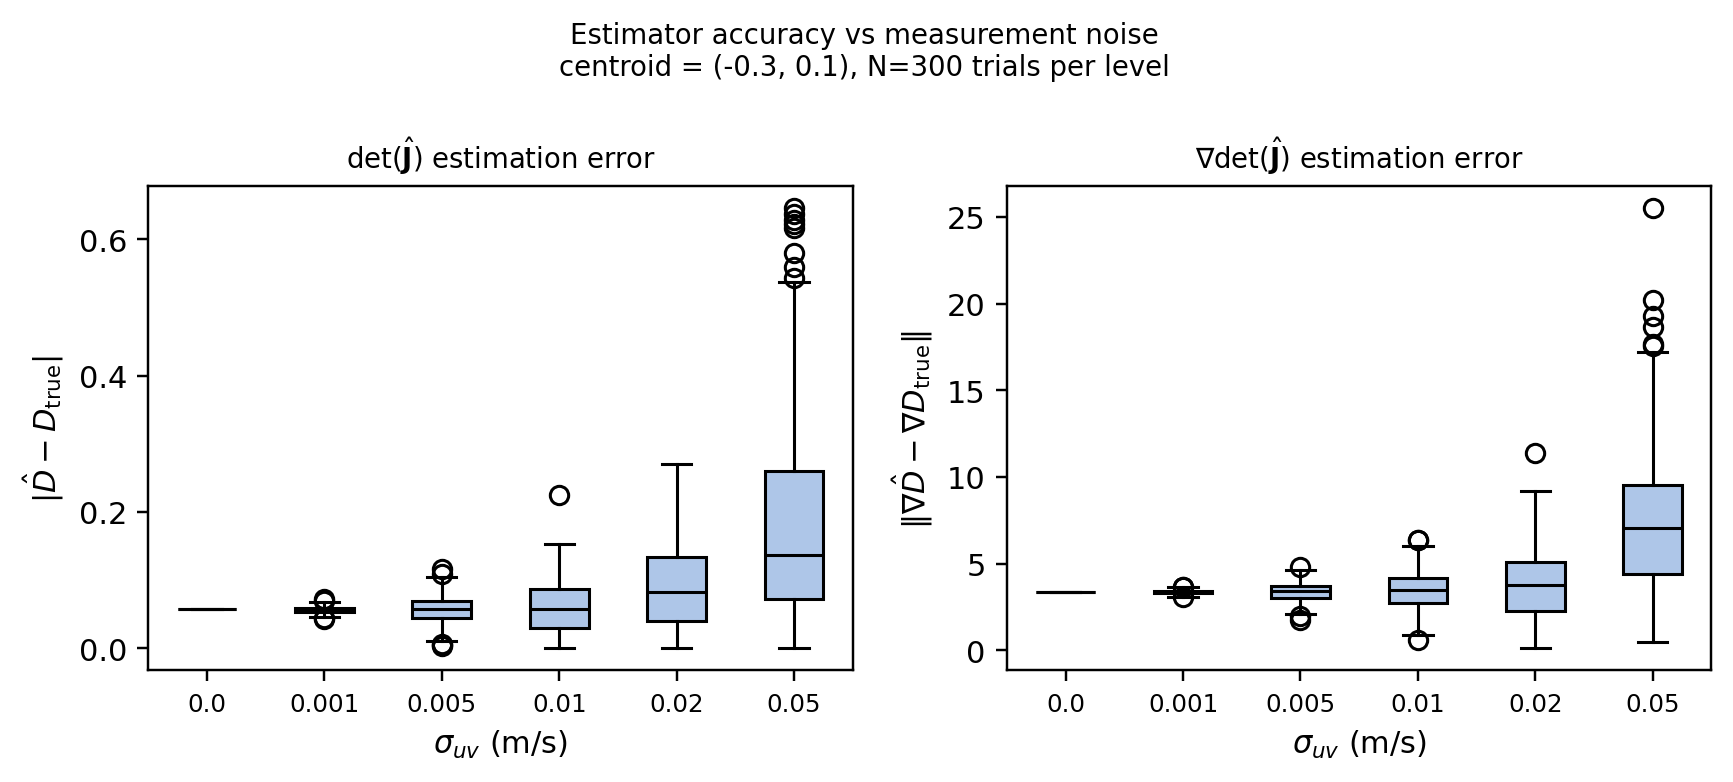
\includegraphics[width=0.45\textwidth]{figures/estimator_accuracy_vs_noise.png}
    % Generated by experiments/estimator_accuracy_sweep.py (CSV data) and
    % experiments/plot_estimator_accuracy.py (figure), under
    % trunk/Python_Simulations/Vector_Fields/VF_Robot/. Review copy in
    % experiments/outputs/estimator_accuracy/.
    \caption{Relative estimation error of $\hat{D}$, $\nabla\hat{D}$, and
    $\hat{\mathbf{H}}_D$ (median over $2 \times 10^5$ noise draws per point;
    shaded interquartile range in (a)) for the steady double gyre of
    Section~\ref{sec:dg_example}, formation held static at the
    strain-region point $\mathbf{p}_c = (-0.35, -0.20)$. (a) Versus measurement noise $\sigma_{uv}$ at the nominal
    formation radius $\rho = 0.075$; the dashed line marks error equal to
    signal magnitude. (b) Versus formation radius $\rho$ at $\sigma_{uv} =
    0.01$; dotted curves are the noise-free truncation floors. $\hat{D}$
    and $\nabla\hat{D}$ exhibit the radius trade-off of (\ref{eq:rho_star});
    $\hat{\mathbf{H}}_D$ is limited by the structural model bias of
    Section~\ref{sec:sensitivity}.}
    \label{fig:est_accuracy}
\end{figure}

Estimator accuracy was measured open loop: the formation was held static
at the strain-region point $\mathbf{p}_c = (-0.35, -0.20)$ of the steady
double gyre, $2 \times 10^5$ independent noise draws were applied per
condition through the same fit used by the controllers, and the estimates
were compared with the analytic values of Appendix~\ref{app:analytic}.
The empirical standard deviation of every fitted coefficient matched the
closed forms of Lemma~\ref{lem:gains} within 0.2\%, and the per-robot
reading error induced by position noise matched the first-order
prediction of Section~\ref{sec:noise_model} within 1\%, confirming that
the two noise channels combine into a single effective measurement noise.

Fig.~\ref{fig:est_accuracy} reports the accuracy of the three navigation
quantities as relative error, the error magnitude divided by the
magnitude of the true quantity; a value of one (dashed line) means the
estimate is as wrong as it is large and carries no directional
information. In Fig.~\ref{fig:est_accuracy}(a) the three curves rise
linearly with $\sigma_{uv}$ and sit stacked a constant factor apart: each
additional derivative order multiplies the noise gain by roughly
$1/\rho$, about 13 at the nominal radius, the ladder of
Lemma~\ref{lem:gains}. Reading off the crossings of the dashed line,
$\hat{D}$ remains informative up to $\sigma_{uv} \approx 0.06$ m/s and
$\nabla\hat{D}$ up to $\sigma_{uv} \approx 0.01$ m/s, while
$\hat{\mathbf{H}}_D$ sits at the line even for the quietest sensors:
below $\sigma_{uv} \approx 0.005$ its error is set by the structural
model bias of Section~\ref{sec:sensitivity}, not by noise.
Fig.~\ref{fig:est_accuracy}(b) fixes $\sigma_{uv} = 0.01$ and varies the
formation radius. Enlarging the ring averages noise over a longer
baseline, so the solid curves fall; the quadratic model simultaneously
fits the curved field more poorly, so the noise-free truncation floors
(dotted) rise. The compromise of (\ref{eq:rho_star}) appears as minima
at $\rho \approx 0.11$ for $\hat{D}$ and $\rho \approx 0.23$ for
$\nabla\hat{D}$. These optima are properties of the double gyre at this
location and noise level, entering through the third-derivative scale
$M_3$; the one-third-power scaling law is general, but a different
field, or a different region of the same field, shifts them.
$\hat{\mathbf{H}}_D$ exhibits no minimum: its floor is radius
independent, as predicted, and no formation size improves it, though its
eigen-directions remain accurate to $0.35^\circ$ on and near the
separatrix and $3.8^\circ$ at the generic test point
(Remark~\ref{rem:eigvec}).

The gradient threshold locates where closed-loop degradation should
begin: at $\sigma_{uv} \approx 0.01$ a single $\nabla\hat{D}$ estimate
is as wrong as it is right, so any one control decision approaches
chance. The closed loop does not extend this limit: the Monte Carlo
sweeps that follow place the 50\% success level of both controllers at
$\sigma_{uv} \approx 0.01$, coinciding with the single-estimate
threshold. Saturation and the per-cycle redraw of the noise bound the
damage of individual bad commands, but they buy no additional margin
for a traverse that requires a long sequence of correct decisions.

\subsection{Separatrix Controller Simulation Results}

\begin{figure}[!t]
    \centering
    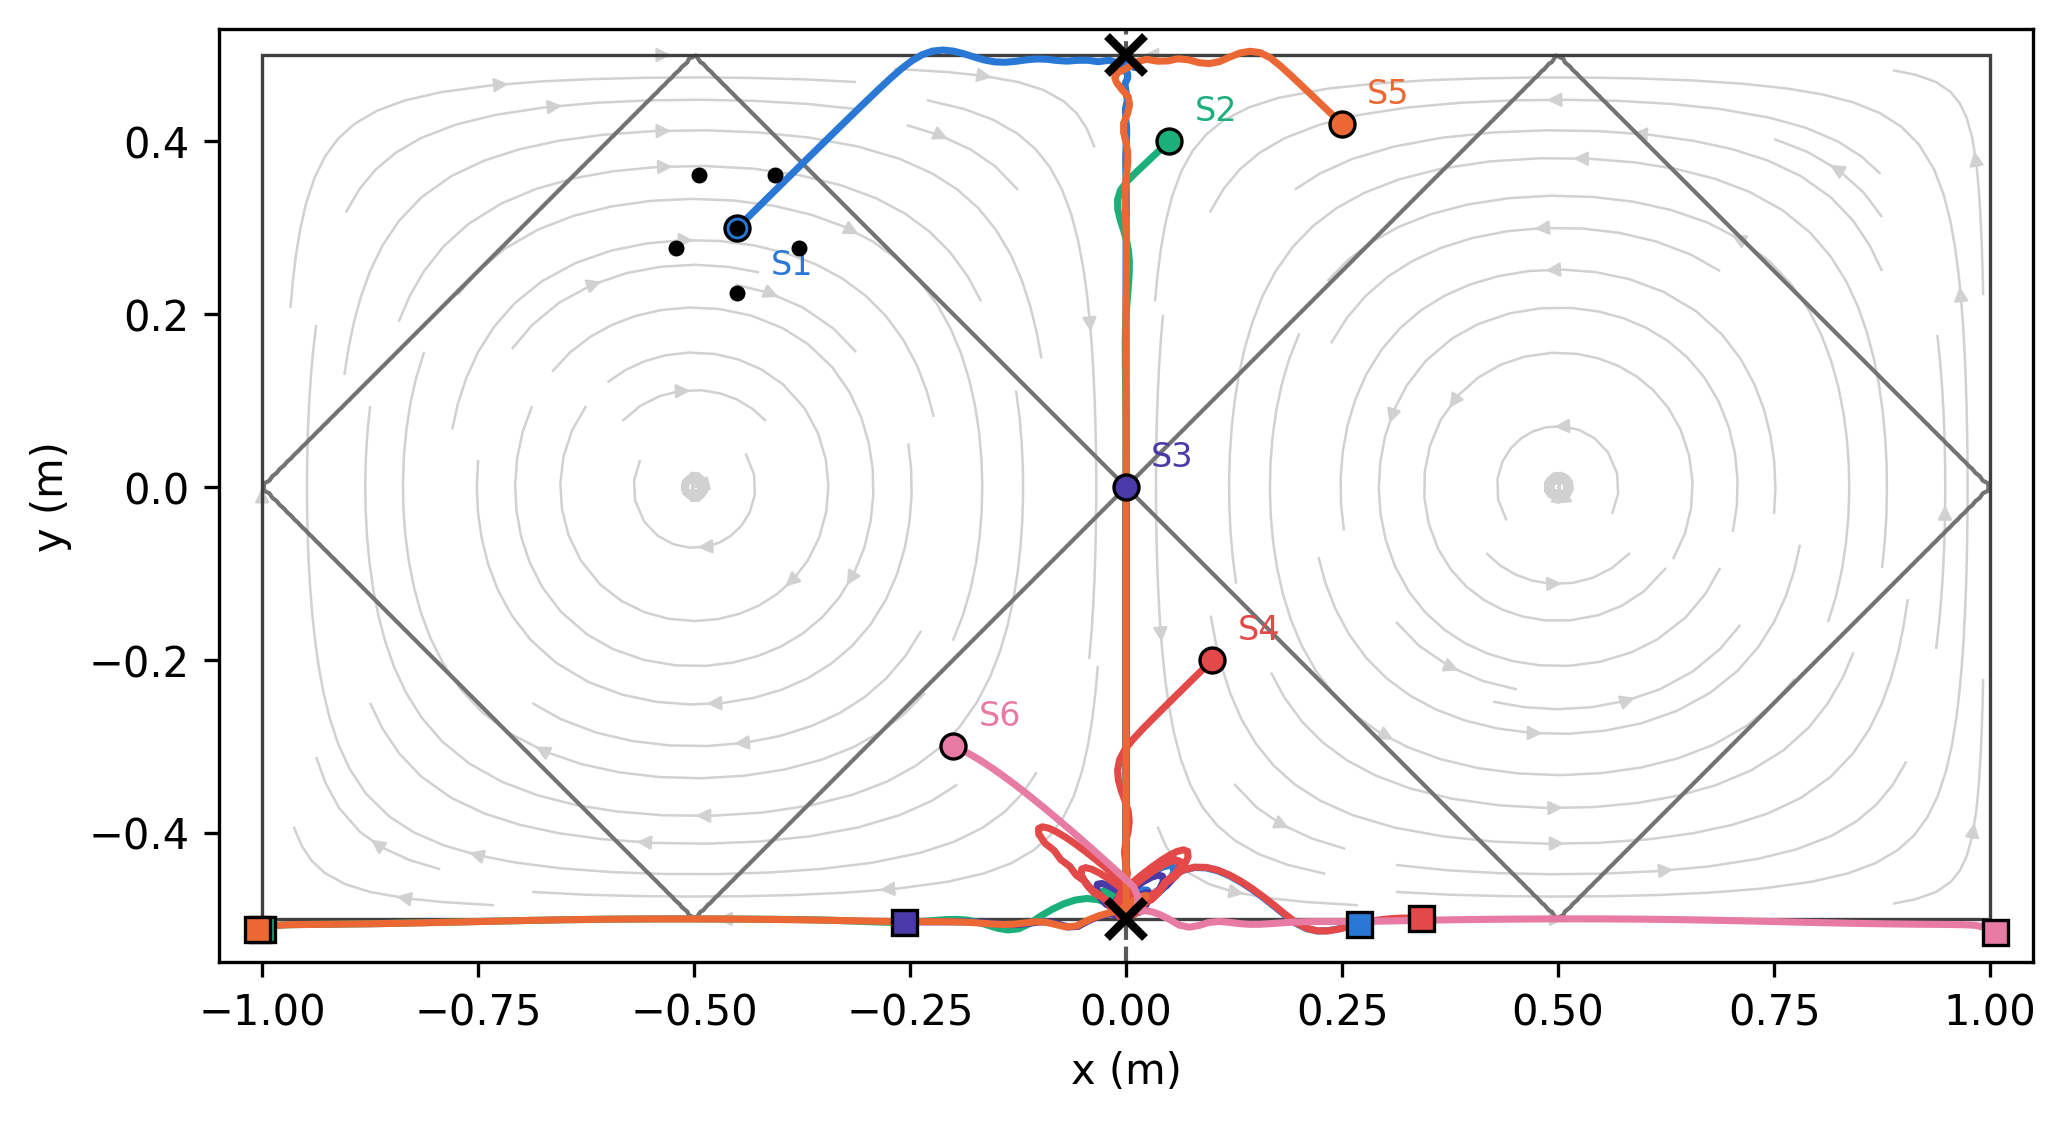
\includegraphics[width=0.45\textwidth]{figures/separatrix_trajectories.png}
    % Generated by experiments/separatrix_clean_runs.py, under
    % trunk/Python_Simulations/Vector_Fields/VF_Robot/. Review copy in
    % experiments/outputs/separatrix_clean/.
    \caption{Separatrix tracker (Logic C) centroid trajectories from six
    initial conditions, noise-free case, overlaid on the double-gyre
    streamlines and the two Okubo-Weiss diamonds. Start points are
    $\bullet$, saddles are $\times$. Every trajectory reaches $x = 0$ and
    continues along the wall trench through the terminal (bottom) saddle
    in both directions; a trial stops at domain exit or 150 steps after
    first saddle contact.}
    \label{fig:sep_trajectories}
\end{figure}

From the six starts of Fig.~\ref{fig:sep_trajectories}, all six reach the
separatrix and pass within 0.02 of the bottom saddle
$\mathbf{p}^*_1$ (closest approach 0.0003--0.0194 across runs). Three of
the six begin already inside the FLOW band and band immediately;
the other three take 6, 18, and 35 steps. Mode occupancy over each run
is FLOW 6--37\%, SLIDE 34--48\%, and ATTRACT 10--24\%, with the
remaining time split between the flow-drift and attract-fallback
refinements of the same three modes; no run spends more than a few
percent of its steps outside these categories. Every run continues past
the terminal saddle rather than stopping there. This traces to the
structural bias of $\hat{\mathbf{H}}_D$ (Section~\ref{sec:sensitivity}):
near the well the estimated eigenvalues are indefinite and roughly an
order of magnitude too small, so the capture test
$\lambda_1\lambda_2 \geq 0$ of Section~\ref{sec:sep_controller} does not
fire even without noise. Section~\ref{sec:discussion} returns to this
behavior, continuous traversal of the separatrix network, with terminal
capture demonstrated as a tightened-threshold special case.

\begin{table}[!t]
\centering
\caption{Separatrix tracker: success rate (traverse) by noise cell,
1000 trials/cell, fixed straddling start $(0, 0.35)$}
\label{tab:sep_success}
\footnotesize
\setlength{\tabcolsep}{4pt}
\begin{tabular}{r|rrrrr}
\hline
$\sigma_{uv}$ \textbackslash\ $\sigma_p$ & 0.000 & 0.005 & 0.010 & 0.020 & 0.050 \\
\hline
0.000 & 100.0 & 64.7 & 45.4 & 36.0 & 18.8 \\
0.001 &  99.3 & 61.9 & 43.7 & 33.8 & 19.9 \\
0.005 &  60.2 & 53.6 & 40.7 & 29.7 & 17.4 \\
0.010 &  43.3 & 40.6 & 39.6 & 28.1 & 18.4 \\
0.020 &  27.6 & 27.5 & 22.9 & 20.4 & 18.4 \\
0.050 &  15.1 & 16.4 & 14.7 & 15.2 & 15.0 \\
0.100 &  13.0 & 15.0 & 13.3 & 14.3 & 13.5 \\
\hline
\end{tabular}
\end{table}

Table~\ref{tab:sep_success} reports traverse success (reaching the
terminal saddle without formation collapse) over the noise grid. At
$\sigma_p = 0$ the rate is a clean step: 100\% through
$\sigma_{uv} = 0.001$, then falling through the 50\% level between
$\sigma_{uv} = 0.005$ and $0.01$, landing at 43.3\% at
$\sigma_{uv} = 0.01$. This coincides with the open-loop
$\nabla\hat{D}$ reliability threshold reported above
($\sigma_{uv} \approx 0.01$, ratio 1.0): saturation and per-cycle
resampling do not extend the noise budget
of a long decision sequence beyond what a single gradient estimate can
support. Position noise degrades the rate along the same curve scaled
by $\|\mathbf{J}\|$, consistent with the effective-noise argument of
Section~\ref{sec:noise_model}: $\sigma_p = 0.01$ alone gives 45.4\%,
close to $\sigma_{uv} = 0.01$ alone at 43.3\%. Beyond the cliff, success
does not fall to zero but levels off near 13--15\%: at this noise level
the controller behaves as an unbiased random walk that occasionally
lands on the saddle by chance, so the straddle-retention metric of
Table~\ref{tab:sep_straddle} is the sharper failure indicator. Tracking
error over the on-trench phase (mean $|x_c|$) rises from 0.002 m at zero
noise to 0.086 m at the $\sigma_{uv} = 0.01$ cliff and saturates near
0.27 m at high noise (comparable to the domain half-width), reflecting
trials that never band at all. Success was independent of initial
heading to within the sampling noise of the sweep (quartile success
74.9--76.2\% at low noise, confirming the isotropy of
Lemma~\ref{lem:gains}).

\begin{table}[!t]
\centering
\caption{Separatrix tracker: straddle retention by noise cell (fraction
of 1000 trials, Michini-comparable metric [14])}
\label{tab:sep_straddle}
\footnotesize
\setlength{\tabcolsep}{4pt}
\begin{tabular}{r|rrrrr}
\hline
$\sigma_{uv}$ \textbackslash\ $\sigma_p$ & 0.000 & 0.005 & 0.010 & 0.020 & 0.050 \\
\hline
0.000 & 1.000 & 0.625 & 0.417 & 0.338 & 0.164 \\
0.005 & 0.560 & 0.493 & 0.365 & 0.272 & 0.157 \\
0.010 & 0.379 & 0.366 & 0.361 & 0.258 & 0.165 \\
0.020 & 0.237 & 0.232 & 0.187 & 0.177 & 0.159 \\
0.050 & 0.126 & 0.137 & 0.112 & 0.128 & 0.122 \\
\hline
\end{tabular}
\end{table}

\subsection{Okubo-Weiss Boundary Tracker Simulation Results}

\begin{figure}[!t]
    \centering
    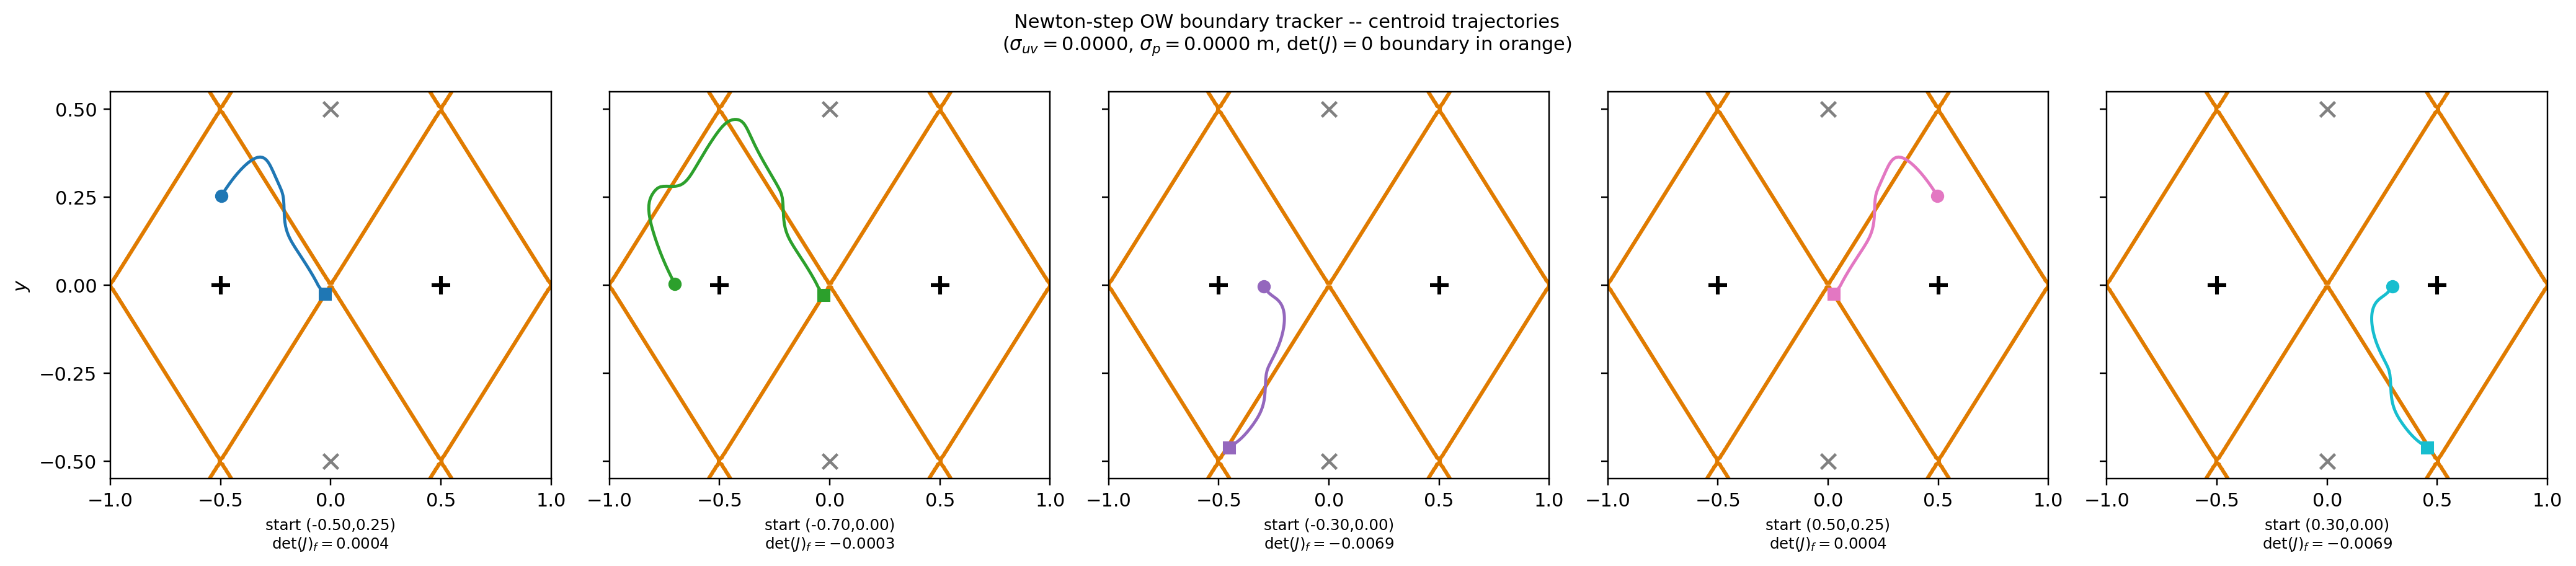
\includegraphics[width=0.45\textwidth]{figures/ow_trajectories.png}
    % Generated by experiments/ow_clean_runs.py, under
    % trunk/Python_Simulations/Vector_Fields/VF_Robot/. Review copy in
    % experiments/outputs/ow_clean/.
    \caption{Okubo-Weiss boundary tracker centroid trajectories from four
    initial conditions, noise-free case, overlaid on $D(\mathbf{p})$
    (red $D>0$ cores, blue $D<0$ exterior) and the diamond boundaries.
    Gyre centers are $+$, diamond corners are $\times$. After lock-on,
    each trajectory follows its diamond edge straight through the
    corners onto the neighboring edge, consistent with the line-network
    structure of $\mathcal{C}$ (Section~\ref{sec:dg_example}).}
    \label{fig:ow_trajectories}
\end{figure}

All four starts of Fig.~\ref{fig:ow_trajectories} lock onto the
boundary in 13--16 steps and hold it: mean $|D|$ on-boundary is
0.0032--0.0075 (0.3--0.8\% of the well depth $\pi^4 A^2 = 0.974$), with
95th-percentile $|D|$ of 0.028--0.039. Runs O3 and O4 each cross one
diamond corner and dwell there for 4--8 steps before continuing on the
new edge; the boundary tracker never turns to circulate a single
diamond, it travels along the connected line network, matching Problem
2's statement in Section~\ref{sec:problem_statement}.

\begin{table}[!t]
\centering
\caption{Okubo-Weiss tracker: success rate (track) by noise cell, 1000
trials/cell, fixed start $(-0.5, 0.25)$}
\label{tab:ow_success}
\footnotesize
\setlength{\tabcolsep}{4pt}
\begin{tabular}{r|rrrrr}
\hline
$\sigma_{uv}$ \textbackslash\ $\sigma_p$ & 0.000 & 0.005 & 0.010 & 0.020 & 0.050 \\
\hline
0.000 & 100.0 & 100.0 & 100.0 &  98.6 &   9.7 \\
0.001 & 100.0 & 100.0 & 100.0 &  98.4 &   9.5 \\
0.005 &  93.8 &  93.7 &  91.6 &  72.8 &   8.1 \\
0.010 &  20.9 &  17.7 &  16.7 &  13.4 &   9.1 \\
0.020 &   8.8 &   8.0 &   9.6 &   7.2 &   7.9 \\
0.050 &   6.6 &   5.5 &   4.4 &   6.7 &   6.0 \\
\hline
\end{tabular}
\end{table}

Table~\ref{tab:ow_success} shows a sharper cliff than the separatrix
tracker: full tolerance through $\sigma_{uv} = 0.001$ regardless of
$\sigma_p$, 93.8\% at $\sigma_{uv} = 0.005$, then a collapse to 20.9\%
at $\sigma_{uv} = 0.01$, the same coordinate as the separatrix
controller's cliff and the same open-loop gradient threshold. Position
noise is tolerated to $\sigma_p = 0.02$ at low $\sigma_{uv}$ (98.6\% at
$\sigma_{uv} = 0$) but the $\sigma_p = 0.05$ column is uniformly under
10\% regardless of $\sigma_{uv}$, since $\sigma_p = 0.05$ alone already
exceeds the reading-error budget the boundary law needs to keep
$|\hat{D}|$ below its lock-on threshold. On-boundary tracking error
($|D(\mathbf{p}_c)|$, mean and 95th percentile) is essentially unchanged
through $\sigma_{uv} = 0.001$ (mean 0.0008--0.0029) and rises steadily
to the well depth scale by $\sigma_{uv} = 0.05$ (mean 0.21, 95th
percentile 0.50). As with the separatrix tracker, success was
independent of initial heading (quartile success 77.6--79.4\% at low
noise).

\subsection{Comparison of the Two Controllers}

Both controllers place their 50\% success level at the same
$\sigma_{uv} \approx 0.01$, the point at which a single
$\nabla\hat{D}$ estimate is as wrong as it is right, reported above in
the estimator-accuracy results. Neither the flow-assisted
separatrix law nor the boundary law's tangential drift extends this
budget: the estimator, not the control law, sets the noise ceiling for
both structures. The boundary tracker's cliff is sharper (100\% to
20.9\% between $\sigma_{uv} = 0.005$ and $0.01$, versus the separatrix
tracker's more gradual 60.2\% to 43.3\% over the same interval) because
tracking $\mathcal{C}$ is a codimension-one regular-level-set problem
that fails outright once $\nabla\hat{D}$ stops resolving the crossing
direction, while the separatrix tracker degrades more gradually because
its FLOW mode can still make progress along the trench using the
ambient flow estimate $\mathbf{f}$ even when $\hat{\mathbf{H}}_D$ is
unreliable. This mirrors the asymmetry in the stability results of
Section~\ref{sec:stability}: the boundary is a single regular curve with
a global certificate; the separatrix is a trench whose capture depends
on curvature the estimator recovers only approximately.


% ---------------------------------------------------------------------------
\section{Discussion}
\label{sec:discussion}

\subsection{Implications for Distributed Eulerian-Structure Following}

The two stability results of Section~\ref{sec:stability} differ in
strength for a structural reason. The Okubo-Weiss boundary is a
codimension-one regular level set: first-order information, a gradient
that does not vanish, fully determines the transversal direction and
yields a global certificate from a single quadratic Lyapunov function.
The separatrix trench lives where that first-order information vanishes
in the normal direction, so any controller and any proof must
synthesize the missing direction from curvature; the eigenstructure
dependence, mode switching, and tube assumptions of
Section~\ref{sec:stab_sep} are the price of that synthesis. The
separatrix result is the more difficult robotics contribution precisely
because the problem is harder; the boundary result is the stronger
theorem precisely because the problem is easier.

The results of Section~\ref{sec:results} show that a six-robot formation
sampling only its own local velocities recovers enough second-order
structure, not the field itself, to find and follow both kinds of
Eulerian feature, with no map, no forecast, and no communication beyond
the single synchronous sample each control cycle already requires. The
$\det(\mathbf{J})$ landscape is what makes this possible: both problems
reduce to following a scalar surrogate field that is computable from
the same twelve fitted coefficients, a trench for the separatrix and a
zero-crossing for the boundary, rather than to any procedure specific
to streamlines or Lagrangian integration. The two controllers are
consequently complementary rather than competing: one tracks a curve
defined by where curvature information vanishes to first order and must
be supplied by the Hessian, the other a curve defined by where the
Hessian itself is unnecessary because the gradient alone is regular
everywhere on it. A team that could estimate both could, in principle,
select which structure to follow from the local field alone, without an
operator choosing in advance.

\subsection{Park versus Traverse: One Threshold, Two Behaviors}
\label{sec:park_vs_traverse}

Theorem~\ref{thm:separatrix} and Remark~\ref{rem:capture_gap} identify
the terminal-capture test $\lambda_1\lambda_2 \geq 0$ as the reason the
deployed controller continues through every saddle in
Section~\ref{sec:results}: the biased $\hat{\mathbf{H}}_D$ makes that
test unreliable exactly where it would need to fire. An estimator-aware
alternative restores capture without touching the transverse Newton
snap, the flow step, or the slide step, using only the two quantities
Section~\ref{sec:sensitivity} shows are linear in the fitted
coefficients and free of the Hessian's structural bias, $\hat{D}$ and
$\hat{\mathbf{g}}$. The \emph{park step} adds a fourth mode, checked
before the FLOW test:
\begin{equation}
    \text{if } \hat{D} < D_{\text{capture}}:\quad
    \dot{\mathbf{p}}_c^{\,\text{des}} =
    -\begin{bmatrix}
        \mathrm{sat}(\hat{g}_x) \\ \mathrm{sat}(\hat{g}_y)
    \end{bmatrix},
    \label{eq:park_step}
\end{equation}
componentwise saturated gradient descent on $\hat{D}$, which converges
to the nearest local minimum of $D$, the flow saddle at the end of the
current trench segment, exactly as Theorem~\ref{thm:attract} predicts
for the exact-estimate case. $D_{\text{capture}}$ is the one-parameter
knob: $D_{\text{capture}} = -\infty$ disables the test and the
controller is trajectory-identical to Logic C (verified in
\textit{separatrix\_logic\_park\_step}, bit-exact off), while a finite
threshold inside the well (here $-0.5$, roughly half the double-gyre
well depth $\pi^4 A^2 \approx 0.974$) parks the team there.
Fig.~\ref{fig:park_vs_traverse} runs both settings from the same start,
noise-free: traverse exits the domain at $(1.00, -0.51)$ after 228
steps, riding the crossing trench as Section~\ref{sec:results}
describes; park reaches the saddle and holds position with zero
tail-position standard deviation over its final 100 steps, settling
0.0124~m from $\mathbf{p}^*_1$. Both runs use the identical estimation
step and the identical selector below the park test; the only
difference is one threshold. This is the practical resolution of
Remark~\ref{rem:capture_gap}: continuation is not a controller limitation
to be designed around so much as the honest behavior of the theorem's
capture test under a real estimator, and a single threshold recovers
whichever behavior a mission calls for, terminal parking at a critical
point or open-ended traversal of the network.

\begin{figure}[!t]
    \centering
    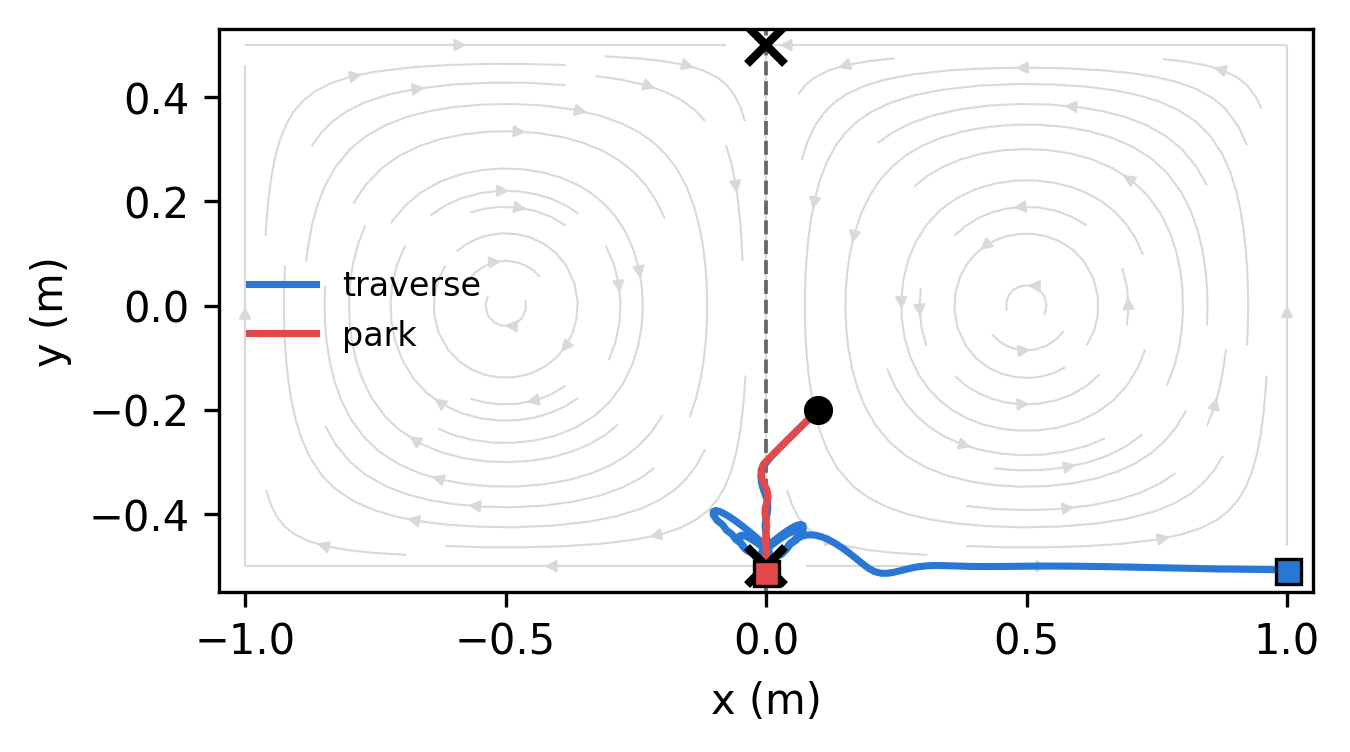
\includegraphics[width=0.45\textwidth]{figures/park_vs_traverse.png}
    % Generated by experiments/park_vs_traverse_demo.py, under
    % trunk/Python_Simulations/Vector_Fields/VF_Robot/. Review copy in
    % experiments/outputs/separatrix_clean/.
    \caption{Park versus traverse from the same start $(0.10, -0.20)$,
    noise-free. Traverse (Logic C) rides the trench through the bottom
    saddle and exits the domain. Park (Logic Park,
    $D_{\text{capture}} = -0.5$) applies the park step
    (\ref{eq:park_step}) once $\hat{D}$ drops below threshold and holds
    the team 0.0124~m from the saddle.}
    \label{fig:park_vs_traverse}
\end{figure}

\subsection{Failure Modes}

% TODO: 4-6 sentences. Cover:
% (1) Estimator ill-conditioning when the formation collapses toward a
%     degenerate configuration (det(Phi) small); propose formation-shape
%     maintenance as mitigation.
% (2) Mode-switching chatter in the separatrix controller when the
%     centroid oscillates across the FLOW-band boundary; discuss the
%     role of the dimensionless threshold eps_dim in damping this.
% (3) Tangential drift in the OW controller can carry the cluster away
%     from the domain boundaries; note this is a simulation artifact
%     (infinite domain).


% ---------------------------------------------------------------------------
\section{Limitations}
\label{sec:limitations}

This paper restricts attention to the static double gyre ($\varepsilon = 0$).
In the time-varying case ($\varepsilon > 0$) the separatrix becomes a
material curve that evolves with the flow, and the det$(\mathbf{J}) = 0$
boundary shifts in time; tracking either structure would require adapting
the control law to account for the flow unsteadiness. This extension is
left to future work.

Results are presented for a single field family (the double gyre). Whether
the separatrix tracker and OW boundary tracker generalize to other fields
with saddle-like or rotation-dominated regions is not addressed here,
though the estimation framework (Section~\ref{sec:estimation}) applies
to any smooth planar vector field.

All results are from simulation only. Hardware validation on the Decabot
testbed is not reported in this paper; it is planned as a follow-on study.

The stability guarantees, and the reported success rates, are local.
Theorem~\ref{thm:separatrix} assumes initialization inside the tube
$T_w$, and all Monte Carlo trials start from a formation straddling the
separatrix. The attract mode converges to the critical set of $D$, which
includes the gyre-center maxima, so a team started deep inside a vortex
core parks at the core rather than on the separatrix: in supplementary
uniform-random-start trials over the domain, roughly half (47.9\%,
$n = 1000$) of starts reached the trench at zero noise. We do not
characterize the basin of attraction of the separatrix; prior
adaptive-navigation primitives [4], [5] likewise report local
convergence without basin estimates.


% ---------------------------------------------------------------------------
\section{Future Work}
\label{sec:future}

Direct extensions of this work include:
\begin{itemize}
    \item \textbf{Time-varying double gyre.} Extending the controllers to
          the $\varepsilon > 0$ case by adding a time-derivative correction
          term to the navigation primitive.
    \item \textbf{Online formation reshaping.} Adapting the pair lengths
          $(L_k)$ and the SAS parameters to improve the conditioning of
          $\boldsymbol{\Phi}$ when the cluster is near a degenerate
          configuration.
    \item \textbf{Hardware deployment.} Validating both controllers on the
          Decabot testbed using the OptiTrack motion-capture system. The
          separatrix and Okubo-Weiss boundaries can be represented by a
          vector field emitted by an on-board computer and sampled by
          the robots' onboard sensors.
    \item \textbf{Extension to 3D.} Generalizing the quadratic estimator
          to three-dimensional fields, which would require at least 10 robots
          per component for full cubic determination, or a reduced-order
          estimator with different assumptions.
\end{itemize}


% ---------------------------------------------------------------------------
\section{Conclusion}
\label{sec:conclusion}

This paper presented a distributed framework for navigating a six-robot
formation along two Eulerian structural boundaries of the double gyre: the
separatrix and the Okubo-Weiss ($\det(\mathbf{J}) = 0$) boundary. A quadratic
estimator using simultaneous measurements from the six robots recovers the
Jacobian, its determinant, gradient, and Hessian at the cluster centroid with
no prior field knowledge. Two parallel adaptive controllers were derived, each
with a Lyapunov stability certificate. Monte Carlo simulation over a
two-dimensional noise sweep quantified the noise robustness of both
controllers.

% TODO: replace the sentences above with specific results once Section IX
% is filled in (success rates, tracking error bounds, noise thresholds).


\appendices

% ---------------------------------------------------------------------------
\section{Double-Gyre Analytic Forms}
\label{app:analytic}

For the steady double gyre with amplitude $A$, $x_f = x + 1$,
$y_f = y + 0.5$, define $s_x = \sin(\pi x_f)$, $c_x = \cos(\pi x_f)$,
$s_y = \sin(\pi y_f)$, $c_y = \cos(\pi y_f)$. The field is
$u = -\pi A s_x c_y$, $v = \pi A c_x s_y$.

The Jacobian entries are
\begin{equation}
    \frac{\partial u}{\partial x} = -\pi^2 A c_x c_y, \quad
    \frac{\partial u}{\partial y} =  \pi^2 A s_x s_y,
\end{equation}
\begin{equation}
    \frac{\partial v}{\partial x} = -\pi^2 A s_x s_y, \quad
    \frac{\partial v}{\partial y} =  \pi^2 A c_x c_y,
\end{equation}
so the flow is divergence free and
\begin{equation}
    D = \det(\mathbf{J})
      = -\pi^4 A^2 \bigl(c_x^2 c_y^2 - s_x^2 s_y^2\bigr)
      = -\frac{\pi^4 A^2}{2}\bigl(\cos 2\pi x_f + \cos 2\pi y_f\bigr),
    \label{eq:det_analytic}
\end{equation}
using $c^2 = (1+\cos 2\alpha)/2$ and $s^2 = (1-\cos 2\alpha)/2$. $D$ is
positive at the gyre centers ($D = \pi^4 A^2$), negative at the corner
saddles ($D = -\pi^4 A^2$), and zero on the diamonds
$x_f \pm y_f \in \tfrac{1}{2} + \mathbb{Z}$, by the factorization
$\cos 2\pi x_f + \cos 2\pi y_f = 2\cos\pi(x_f+y_f)\cos\pi(x_f-y_f)$.

Differentiating (\ref{eq:det_analytic}),
\begin{equation}
    \nabla D = \pi^5 A^2
    \begin{bmatrix} \sin 2\pi x_f \\ \sin 2\pi y_f \end{bmatrix},
    \qquad
    \mathbf{H}_D = 2\pi^6 A^2
    \begin{bmatrix} \cos 2\pi x_f & 0 \\ 0 & \cos 2\pi y_f \end{bmatrix}.
    \label{eq:gradhess_analytic}
\end{equation}
The Hessian is diagonal everywhere, so $D$ is additively separable in
$x_f$ and $y_f$, which is what makes the trench normal form of
Assumption~\ref{ass:trench} exact for this field. The vorticity is
$\omega = -2\pi^2 A s_x s_y$, which vanishes on the separatrix
$x_f = 1$; there $\mathbf{J}$ is symmetric and $\sqrt{-D}$ is the
exact instantaneous strain rate. The Okubo-Weiss parameter is
$Q = -D$ by incompressibility, so the $Q = 0$ and $D = 0$ contours
coincide.


% ---------------------------------------------------------------------------
\section{Pentagon Cluster Kinematics}
\label{app:kinematics}

\subsection{Forward Kinematics}

The pentagon-of-pairs cluster has 6 robots indexed $i = 1, \ldots, 6$, arranged
as three pairs. Pair $k$ ($k = 1, 2, 3$) consists of robots $2k-1$ and $2k$.
The midpoint of pair $k$ is $\mathbf{m}_k = (\mathbf{p}_{2k-1} +
\mathbf{p}_{2k})/2$. The three midpoints form a triangle; the centroid of that
triangle is $\mathbf{p}_c = (\mathbf{m}_1 + \mathbf{m}_2 + \mathbf{m}_3)/3$.

The SAS parameters of the midpoint triangle are defined as in the three-robot
case: $p_1 = \|\mathbf{m}_2 - \mathbf{m}_1\|$, $q_1 = \|\mathbf{m}_3 -
\mathbf{m}_2\|$, and $\beta_1$ is the interior angle at $\mathbf{m}_2$.
The cluster heading $\theta_c = \text{atan2}(m_{2,y} - m_{1,y},
m_{2,x} - m_{1,x})$.

Each pair is described by its half-length $L_k/2$ and orientation angle
$\psi_k$, so the two robots in pair $k$ are at $\mathbf{m}_k \pm (L_k/2)
(\cos\psi_k, \sin\psi_k)^\top$.

The full 12-state cluster configuration is
$(x_c, y_c, \theta_c, p_1, \beta_1, q_1, L_2, \psi_2, L_3, \psi_3,
L_4, \psi_4)$, where pair 1 uses $L_1$ fixed and $\psi_1 = \theta_c$ by
convention.

\subsection{Inverse Kinematics}

Given the 12-state cluster configuration, the six robot positions are recovered
by:
\begin{enumerate}
    \item Constructing the midpoint triangle from $(p_1, \beta_1, q_1)$ in
          a local frame (following the same procedure as the three-robot
          cluster in Appendix B of [6]).
    \item Rotating and translating to the global frame using $\theta_c$,
          $x_c$, $y_c$.
    \item Placing each pair of robots by offsetting from the midpoint along
          $(\cos\psi_k, \sin\psi_k)$ by $L_k/2$ in each direction.
\end{enumerate}

\subsection{Inverse Kinematic Jacobian}

The $12 \times 12$ inverse kinematic Jacobian maps desired cluster state
velocities $\dot{\boldsymbol{\xi}}$ to robot velocity commands
$(\dot{x}_1, \dot{y}_1, \ldots, \dot{x}_6, \dot{y}_6)^\top$:
\begin{equation}
    \begin{bmatrix} \dot{x}_1 \\ \dot{y}_1 \\ \vdots \\
    \dot{x}_6 \\ \dot{y}_6 \end{bmatrix}
    =
    \mathbf{J}_c^{-1}
    \begin{bmatrix} \dot{x}_c \\ \dot{y}_c \\ \dot{\theta}_c \\
    \dot{p}_1 \\ \dot{\beta}_1 \\ \dot{q}_1 \\
    \dot{L}_2 \\ \dot{\psi}_2 \\ \dot{L}_3 \\ \dot{\psi}_3 \\
    \dot{L}_4 \\ \dot{\psi}_4 \end{bmatrix},
    \label{eq:inv_kin_jac}
\end{equation}
where $\mathbf{J}_c^{-1}$ is a $12 \times 12$ matrix of partial derivatives
$\partial (x_i, y_i) / \partial \xi_j$ computed analytically from the inverse
kinematics. The explicit entries are omitted here for brevity; the
implementation is in \textit{pentagon\_kinematics.py}.


% ---------------------------------------------------------------------------
\begin{thebibliography}{99}

\bibitem{1} G. Haller and G. Yuan, "Lagrangian coherent structures and mixing
in two-dimensional turbulence," \textit{Physica D: Nonlinear Phenomena},
vol. 147, no. 3-4, pp. 352--370, 2000.

\bibitem{2} T. Peacock and G. Haller, "Lagrangian coherent structures: The
hidden skeleton of fluid flows," \textit{Physics Today}, vol. 66, no. 2,
pp. 41--47, 2013.

\bibitem{3} S. C. Shadden, F. Lekien, and J. E. Marsden, "Definition and
properties of Lagrangian coherent structures from finite-time Lyapunov
exponents in two-dimensional aperiodic flows," \textit{Physica D}, vol. 212,
no. 3-4, pp. 271--304, 2005.

\bibitem{4} R. T. McDonald, C. A. Kitts, and M. A. Neumann, "Navigation of
scalar fronts with multirobot clusters in simulation and experiment,"
\textit{IEEE Systems Journal}, vol. 14, no. 3, pp. 3755--3766, 2020.

\bibitem{5} C. A. Kitts, R. T. McDonald, and M. A. Neumann, "Adaptive
navigation control primitives for multirobot clusters: Extrema finding,
contour following, ridge/trench following, and saddle point station keeping,"
\textit{IEEE Access}, vol. 6, pp. 17625--17642, 2018.

\bibitem{6} C. Waight and C. A. Kitts, "Adaptive navigation of multirobot
systems to critical points in 2D vector fields," \textit{IEEE/ASME Transactions
on Mechatronics}, % TODO: add volume, issue, page range, year once published.

\bibitem{7} A. Okubo, "Horizontal dispersion of floatable particles in the
vicinity of velocity singularities such as convergences," \textit{Deep-Sea
Research}, vol. 17, no. 3, pp. 445--454, 1970.

\bibitem{8} J. Weiss, "The dynamics of enstrophy transfer in two-dimensional
hydrodynamics," \textit{Physica D: Nonlinear Phenomena}, vol. 48, no. 2-3,
pp. 273--294, 1991.

\bibitem{9} B.-L. Hua and P. Klein, "An exact criterion for the stirring
properties of nearly two-dimensional turbulence," \textit{Physica D}, vol. 113,
no. 1, pp. 98--110, 1998.

\bibitem{10} P. Ögren, E. Fiorelli, and N. E. Leonard, "Cooperative control
of mobile sensor networks: Adaptive gradient climbing in a distributed
environment," \textit{IEEE Transactions on Automatic Control}, vol. 49, no. 8,
pp. 1292--1302, 2004.

\bibitem{11} L. Briñón-Arranz, A. Renzaglia, and L. Schenato, "Multirobot
symmetric formations for gradient and Hessian estimation with application to
source seeking," \textit{IEEE Transactions on Robotics}, vol. 35, no. 3,
pp. 782--789, 2019.

\bibitem{12} C. A. Kitts and I. Mas, "Cluster space specification and control
of mobile multirobot systems," \textit{IEEE/ASME Transactions on Mechatronics},
vol. 14, no. 2, pp. 207--218, 2009.

\bibitem{13} T. Adamek, C. A. Kitts, and I. Mas, "Gradient-based cluster space
navigation for autonomous surface vessels," \textit{IEEE/ASME Transactions on
Mechatronics}, vol. 20, no. 2, pp. 506--518, 2014.

\bibitem{14} M. Michini, M. A. Hsieh, E. Forgoston, and I. B. Schwartz,
"Robotic tracking of coherent structures in flows," \textit{IEEE Transactions
on Robotics}, vol. 30, no. 3, pp. 593--603, 2014.

\bibitem{15} D. Kularatne and M. A. Hsieh, "Tracking attracting manifolds in
flows," \textit{Autonomous Robots}, vol. 41, no. 8, pp. 1575--1588, 2017.

\bibitem{16} G. Knizhnik, P. Li, X. Yu, and M. A. Hsieh, "Flow-based control
of marine robots in gyre-like environments," in \textit{Proc. 2022 Int. Conf.
on Robotics and Automation (ICRA)}, pp. 3047--3053, 2022.

% TODO: add any additional references as needed (Haller 2015 coherent structure
% review, Hunt Q-criterion 1988, additional cluster space references, etc.).

\bibitem{17} M. Serra and G. Haller, "Objective Eulerian coherent
structures," \textit{Chaos: An Interdisciplinary Journal of Nonlinear
Science}, vol. 26, no. 5, p. 053110, 2016.

\bibitem{18} Y. N. Dauphin, R. Pascanu, C. Gulcehre, K. Cho, S. Ganguli,
and Y. Bengio, "Identifying and attacking the saddle point problem in
high-dimensional non-convex optimization," in \textit{Advances in Neural
Information Processing Systems}, vol. 27, pp. 2933--2941, 2014.

\bibitem{19} P. J. Nolan, M. Serra, and S. D. Ross, "Finite-time Lyapunov
exponents in the instantaneous limit and material transport,"
\textit{Nonlinear Dynamics}, vol. 100, no. 4, pp. 3825--3852, 2020.

\end{thebibliography}


\begin{IEEEbiography}[{
\includegraphics[width=1in,height=1.25in,clip,keepaspectratio]{figures/cwaight.jpg}}]{Christopher Waight}
% TODO: insert bio.
\end{IEEEbiography}

\begin{IEEEbiography}[{
\includegraphics[width=1in,height=1.25in,clip,keepaspectratio]{figures/ckitts.jpg}}]{Christopher A. Kitts}
% TODO: insert bio.
\end{IEEEbiography}

\end{document}
